% =====================================================================
%  W1D3 -- Control in Robotic & Mechatronic Systems
%  Mechatronics and Robotics Engineering (50 h), Week 1 Day 3
%  Build: cd robotics && ./compile.sh w1d3
%  Plot data: data/*.dat (new ones from data/gen_data.py, others reused from day2/data)
% =====================================================================
\documentclass[aspectratio=169,10pt]{beamer}
\usetheme{mekatronik}
\renewcommand{\coursetitle}{Mechatronics and Robotics Engineering (50 h)}
\setweek{1}
\setday{3}{Control in Robotic Systems}
\title[Control in Robotic Systems]{Control in Robotic \& Mechatronic Systems}
\subtitle{Block diagrams \& state space \textbullet\ Bode plots \textbullet\ PID control \textbullet\ Stability \& performance}
\author{Mechatronics and Robotics Engineering Programme}
\institute{Week 1 \textperiodcentered{} Day 3}
\date{2 weeks \textperiodcentered{} 10 days \textperiodcentered{} 50 hours}

% ------------------------------------------------------------- helpers
\tikzset{
  blk/.style={draw=mkBlue,fill=mkPale,thick,rounded corners=1pt,minimum height=7mm,minimum width=10mm,font=\scriptsize,align=center},
  blko/.style={blk,draw=mkOrange,fill=mkCream},
  sum/.style={draw=mkBlue,thick,circle,inner sep=0pt,minimum size=4mm,fill=white},
  sig/.style={-{Latex[length=2mm]},thick,mkNavy},
  lbl/.style={font=\scriptsize,text=mkNavy},
}
\newcommand{\further}[1]{{\color{mkGray}\scriptsize\textbf{Going further:} #1}}

\begin{document}

\begin{frame}[plain]\titlepage\end{frame}

% =====================================================================
\begin{frame}{Agenda and learning outcomes}
\begin{columns}[T]
\column{.50\textwidth}
\footnotesize
\begin{tabular}{@{}lp{4.4cm}r@{}}
\toprule
\textbf{Code} & \textbf{Session} & \textbf{Time}\\
\midrule
2.3 & Block diagrams, feedback and state-space basics & 1.0\,h\\
2.4 & Frequency response and Bode plots & 1.0\,h\\
2.5 & PID control: P/I/D effects, tuning, windup, feedforward & 1.5\,h\\
2.6 & Stability and performance: specs, steady-state error, margins, bandwidth & 1.5\,h\\
\midrule
 & \textbf{Net teaching time} (+ short breaks) & \textbf{5.0\,h}\\
\bottomrule
\end{tabular}\\[2mm]
\begin{notebox}
Running example all day: \hl{one robot joint} (motor + gearbox + link). Refresher boxes: matrices, sine response, decibels. Small grey ``Going further'' items are optional.
\end{notebox}
\column{.47\textwidth}
\begin{defbox}[By the end of today you can \ldots]
\footnotesize
\checkitem\ \textbf{draw} a feedback loop as a block diagram and \textbf{reduce} it to one transfer function\\[2pt]
\checkitem\ \textbf{write} a simple system in state-space form\\[2pt]
\checkitem\ \textbf{read} a Bode plot (dB, degrees) and \textbf{spot} a resonance\\[2pt]
\checkitem\ \textbf{explain} what P, I and D do to a robot joint and \textbf{pick} starting gains\\[2pt]
\checkitem\ \textbf{judge} a loop from overshoot, steady-state error, phase/gain margin and bandwidth
\end{defbox}
\end{columns}
\end{frame}

% =====================================================================
\begin{frame}{What we learned so far (1/2): the robot joint hardware}
\begin{columns}[T]
\column{.52\textwidth}
\centering
\begin{tikzpicture}[font=\scriptsize]
  % motor
  \draw[thick,fill=mkPale,draw=mkBlue] (0,0) rectangle (1.4,1.2); \node[align=center] at (.7,.6) {motor\\$J_m$};
  \draw[very thick,mkNavy] (1.4,.6)--(2.0,.6);
  % gearbox
  \draw[thick,fill=mkCream,draw=mkOrange] (2.0,.1) rectangle (3.1,1.1); \node[align=center] at (2.55,.6) {gear\\$N{:}1$};
  \draw[very thick,mkNavy] (3.1,.6)--(3.6,.6);
  % link
  \fill[mkBlue] (3.6,.6) circle (.12);
  \draw[line width=5pt,mkMid,rounded corners] (3.6,.6)--(5.6,1.6);
  \fill[mkOrange] (5.6,1.6) circle (.18); \node[right] at (5.75,1.6) {payload};
  \node at (4.5,.55) {link $J_L$};
  \draw[-{Latex},mkOrange,thick] (3.95,1.15) arc (60:20:.5) node[right]{$\theta$};
  \node[mkGray,align=center] at (2.6,-.45) {amplifier sends current $i$ $\Rightarrow$ torque $k_t i$};
\end{tikzpicture}\\[3mm]
\begin{eqbox}
\[
J_{\mathrm{eq}}=J_m+\frac{J_L}{N^2}
\]
\end{eqbox}
\column{.45\textwidth}
\small
From W1D1--W1D2:
\begin{itemize}
  \item Electric motors make torque $T=k_t\,i$; back-EMF $e=k_e\,\omega$.
  \item Gearboxes trade speed for torque; the load inertia is seen \hl{divided by $N^2$} at the motor.
  \item Backlash and elasticity (harmonic drive!) make the joint less ``perfect''.
  \item Sizing: peak and RMS torque, speed, thermal limits.
\end{itemize}
\footnotesize
Today we ask: \hl{how do we make this joint go exactly where we want?}
\end{columns}
\end{frame}

% ---------------------------------------------------------------------
\begin{frame}{What we learned so far (2/2): models and transfer functions}
\begin{columns}[T]
\column{.48\textwidth}
\small
\begin{itemize}
  \item Physics $\Rightarrow$ ODE (mass--spring--damper, motor).
  \item Laplace: ODE $\Rightarrow$ algebra; $G(s)=Y(s)/U(s)$.
  \item \term{Poles} = roots of the denominator: they decide stability and speed.
  \item First order: $K,\tau$ (63\,\% at $t=\tau$).
  \item Second order: $\omega_n$, $\zeta$ (bounciness).
\end{itemize}
\begin{eqbox}
\[
G_{\mathrm{joint}}(s)=\frac{\Theta(s)}{T(s)}=\frac{1}{Js^2+Bs}
\]
\end{eqbox}
\footnotesize Torque in, angle out. Today: $J=0.5$\,kg\,m$^2$, $B=0.1$\,Nm\,s/rad (joint side).
\column{.5\textwidth}
\centering
\begin{tikzpicture}
\begin{axis}[mkplot,width=7.2cm,height=5.0cm,xlabel={time $\omega_n t$},ylabel={step response $y$},xmin=0,xmax=12,ymin=0,ymax=1.6,
  legend pos=south east,legend cell align=left]
  \addplot[mkSky,very thick,domain=0:12,samples=100] {1-exp(-x)}; \addlegendentry{1st order}
  \addplot[mkOrange,thick,domain=0:12,samples=200] {1-exp(-0.2*x)/sqrt(1-0.04)*sin(deg(sqrt(1-0.04)*x)+acos(0.2))}; \addlegendentry{2nd, $\zeta=0.2$}
  \addplot[mkBlue,very thick,domain=0:12,samples=200] {1-exp(-0.7*x)/sqrt(1-0.49)*sin(deg(sqrt(1-0.49)*x)+acos(0.7))}; \addlegendentry{2nd, $\zeta=0.7$}
  \addplot[mkGray,dashed,domain=0:12] {1};
\end{axis}
\end{tikzpicture}\\
\footnotesize Same speed scale, very different shapes: $\zeta$ sets the overshoot.
\end{columns}
\end{frame}

% =====================================================================
\section{2.3 Block Diagrams, Feedback and State-Space Basics}
% =====================================================================

\begin{frame}{Why does a robot need feedback at all?}
\begin{columns}[T]
\column{.42\textwidth}
\centering
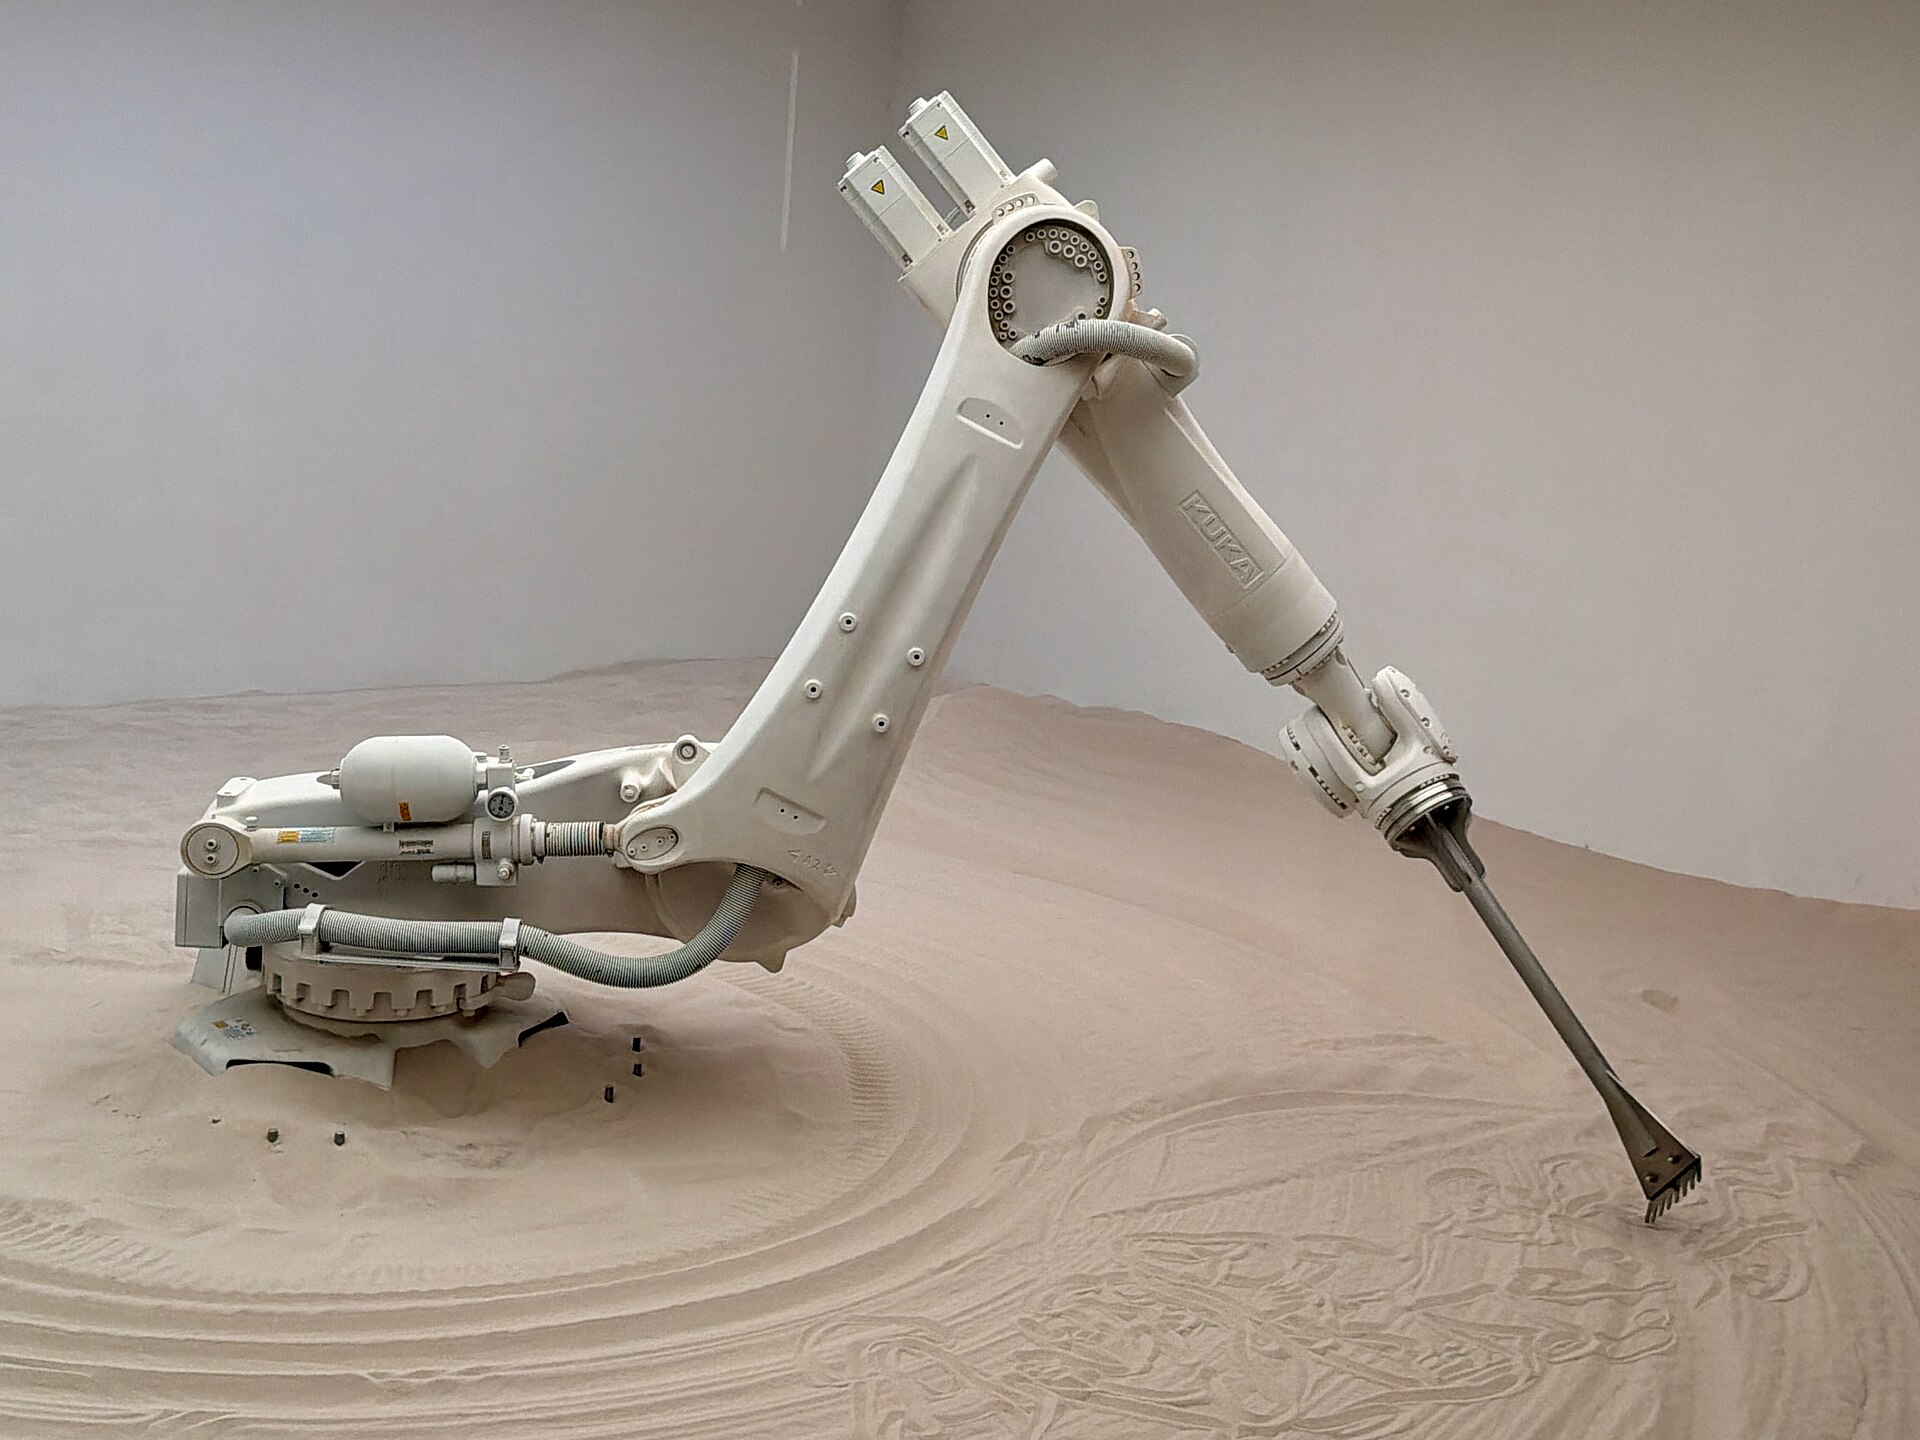
\includegraphics[width=\linewidth]{../../figures/d4_kuka_robot.jpg}\\
\credit{Oleg Yunakov, CC BY-SA 4.0, via Wikimedia Commons}\\[1mm]
\footnotesize\raggedright
An industrial arm repeats a pose to about $\pm0.05$\,mm while payload, temperature and friction change.
\column{.55\textwidth}
\small
\textbf{Open loop}: send a fixed torque profile and hope.
\begin{center}
\begin{tikzpicture}[node distance=6mm]
  \node[blk] (C) {command\\profile};
  \node[blko,right=of C] (G) {joint\\$G(s)$};
  \draw[sig] ($(C.west)-(6mm,0)$) node[left,lbl]{$\theta_r$}--(C);
  \draw[sig] (C)--(G) node[midway,above,lbl]{$T$};
  \draw[sig] (G)--++(12mm,0) node[right,lbl]{$\theta$ ?};
  \draw[sig,mkRed] ($(G.north)+(0,6mm)$) node[above,lbl,text=mkRed]{payload, gravity, friction}--(G);
\end{tikzpicture}
\end{center}
\footnotesize
\begin{itemize}
  \item The joint is a double integrator: a tiny torque error grows into a \hl{large drift} in angle.
  \item The model is never exact (payload unknown, friction varies, gear wears).
  \item \textbf{Closed loop}: measure $\theta$ with an \term{encoder}, compare with $\theta_r$, correct the torque.
\end{itemize}
\end{columns}
\end{frame}

% ---------------------------------------------------------------------
\begin{frame}{Feedback: the cruise-control story}
\centering
\begin{tikzpicture}[node distance=8mm,scale=.85,transform shape]
  \node[sum] (s1) {};
  \node[blk,right=of s1,minimum width=22mm] (C) {controller\\(cruise ECU)};
  \node[sum,right=12mm of C] (s2) {};
  \node[blko,right=of s2,minimum width=22mm] (G) {engine + car};
  \node[blk,below=6mm of C,minimum width=22mm] (M) {speedometer};
  \draw[sig] ($(s1.west)-(16mm,0)$) node[above right,lbl]{set speed $r$} --(s1) node[pos=.85,above,lbl]{$+$};
  \draw[sig] (s1)--(C) node[midway,above,lbl]{error $e$};
  \draw[sig] (C)--(s2) node[midway,above,lbl]{throttle $u$};
  \draw[sig] (s2)--(G);
  \draw[sig] (G)--++(22mm,0) node[above left,lbl]{speed $y$};
  \draw[sig] ($(s2.north)+(0,8mm)$) node[above,lbl]{hill / wind $d$}--(s2);
  \fill ($(G.east)+(12mm,0)$) circle (1.2pt);
  \draw[sig] ($(G.east)+(12mm,0)$) |- (M);
  \draw[sig] (M) -| (s1) node[pos=.95,left,lbl]{$-$};
\end{tikzpicture}\\[2mm]
\begin{columns}[T]
\column{.48\textwidth}
\footnotesize
\begin{itemize}
  \item \textbf{Measure} the speed, \textbf{compare} with the set speed, \textbf{correct} the throttle.
  \item Robot joint: set speed $\to$ target angle, speedometer $\to$ encoder, throttle $\to$ motor current.
  \item Feedback fights disturbances \hl{it does not know about}.
\end{itemize}
\column{.5\textwidth}
\begin{defbox}[Worked example: P control only]
\footnotesize
Controller $u=K_p\,e$. Car: 2\,km/h per \% throttle ($G=2$); $K_p=4.5$\,\%/(km/h) $\Rightarrow$ loop gain $L=K_pG=9$.
\begin{enumerate}
  \item $y=\frac{L}{1+L}\,r=\frac{9}{10}\cdot100=90$\,km/h
  \item A \hl{10\,km/h offset} remains: P alone needs an error to push.
\end{enumerate}
\end{defbox}
\end{columns}
\end{frame}

% ---------------------------------------------------------------------
\begin{frame}{Block diagrams: the four building blocks}
\centering
\begin{tikzpicture}[font=\small]
  % signal
  \draw[sig] (0,0)--(2,0) node[midway,above,lbl]{$u(t)$, $U(s)$};
  \node[align=center,font=\scriptsize,text=mkGray] at (1,-.7) {\textbf{signal}\\a quantity with units\\(V, A, Nm, rad)};
  % block
  \node[blk,minimum width=14mm] (b) at (4.2,0) {$G(s)$};
  \draw[sig] (3,0)--(b) node[pos=.3,above,lbl]{$U$}; \draw[sig] (b)--(5.6,0) node[pos=.7,above,lbl]{$Y$};
  \node[align=center,font=\scriptsize,text=mkGray] at (4.3,-.7) {\textbf{block}\\$Y=G\,U$\\(multiply)};
  % summing junction
  \node[sum] (s) at (7.6,0) {};
  \draw[sig] (6.7,0)--(s) node[pos=.6,above,lbl]{$+$}; \draw[sig] (7.6,.8)--(s) node[pos=.5,right,lbl]{$-$};
  \draw[sig] (s)--(8.5,0);
  \node[lbl] at (6.6,.25) {$a$}; \node[lbl] at (7.85,.85) {$b$}; \node[lbl] at (8.75,0) {$a-b$};
  \node[align=center,font=\scriptsize,text=mkGray] at (7.6,-.7) {\textbf{summing junction}\\add / subtract\\(same units!)};
  % pick-off
  \draw[sig] (10,0)--(11.7,0); \fill (10.8,0) circle (1.5pt); \draw[sig] (10.8,0)--(10.8,.8);
  \node[align=center,font=\scriptsize,text=mkGray] at (10.85,-.7) {\textbf{pick-off point}\\copy a signal\\(a sensor)};
\end{tikzpicture}\\[4mm]
\begin{columns}[T]
\column{.5\textwidth}
\small
A \term{block diagram} is a map of how signals flow and change. Each block is a transfer function from Day 2; the arrows are signals.
\begin{itemize}
  \item Arrows have one direction: cause $\to$ effect.
  \item Feedback = an arrow going \hl{back} to an earlier summing junction.
\end{itemize}
\column{.47\textwidth}
\centering
\begin{tikzpicture}[node distance=5mm]
  \node[blk] (a) {amplifier\\$K_a$};
  \node[blk,right=of a] (m) {motor\\$k_t$};
  \node[blko,right=of m] (j) {joint\\$\frac{1}{Js^2+Bs}$};
  \draw[sig] ($(a.west)-(5mm,0)$) node[left,lbl]{$v$}--(a);
  \draw[sig] (a)--(m) node[midway,above,lbl]{$i$};
  \draw[sig] (m)--(j) node[midway,above,lbl]{$T$};
  \draw[sig] (j)--++(9mm,0) node[right,lbl]{$\theta$};
\end{tikzpicture}\\[1mm]
\footnotesize Series blocks multiply: $\Theta/V=K_a\,k_t/(Js^2+Bs)$.
\end{columns}
\end{frame}

% ---------------------------------------------------------------------
\begin{frame}{Block-diagram algebra}
\centering
\begin{tikzpicture}[node distance=5mm,font=\scriptsize,scale=.9,transform shape]
  \node[lbl,font=\scriptsize\bfseries,anchor=west] at (-0.4,1.0) {Series};
  \node[blk] (a1) at (0.8,0) {$G_1$}; \node[blk,right=of a1] (a2) {$G_2$};
  \draw[sig] (-.2,0)--(a1); \draw[sig] (a1)--(a2); \draw[sig] (a2)--++(7mm,0);
  \node at (3.6,0) {$\Longleftrightarrow$};
  \node[blko] (a3) at (5.0,0) {$G_1G_2$}; \draw[sig] (4.1,0)--(a3); \draw[sig] (a3)--++(7mm,0);
  \node[lbl,font=\scriptsize\bfseries,anchor=west] at (7.4,1.0) {Parallel};
  \node[blk] (b1) at (9.0,.45) {$G_1$}; \node[blk] (b2) at (9.0,-.45) {$G_2$};
  \node[sum] (bs) at (10.2,0) {}; \fill (8.2,0) circle (1pt);
  \draw[sig] (7.7,0)--(8.2,0) |- (b1); \draw[sig] (8.2,0) |- (b2);
  \draw[sig] (b1) -| (bs); \draw[sig] (b2) -| (bs); \draw[sig] (bs)--++(5mm,0);
  \node at (11.1,0) {$\Leftrightarrow$};
  \node[blko] (b3) at (12.6,0) {$G_1+G_2$}; \draw[sig] (11.5,0)--(b3); \draw[sig] (b3)--++(7mm,0);
  \node[lbl,font=\scriptsize\bfseries,anchor=west] at (-0.4,-1.3) {Negative feedback};
  \node[sum] (cs) at (0.6,-2.2) {}; \node[blk,right=of cs] (c1) {$G_1$};
  \node[blk,below=4mm of c1] (c2) {$G_2$};
  \draw[sig] (-.2,-2.2)--(cs) node[pos=.6,above]{$+$}; \draw[sig] (cs)--(c1);
  \draw[sig] (c1)--++(10mm,0) coordinate (co); \fill ($(c1.east)+(5mm,0)$) circle (1pt);
  \draw[sig] ($(c1.east)+(5mm,0)$) |- (c2); \draw[sig] (c2) -| (cs) node[pos=.9,left]{$-$};
  \node at (3.6,-2.2) {$\Longleftrightarrow$};
  \node[blko] (c3) at (5.2,-2.2) {$\dfrac{G_1}{1+G_1G_2}$}; \draw[sig] (4.1,-2.2)--(c3); \draw[sig] (c3)--++(9mm,0);
  \node[lbl,font=\scriptsize\bfseries,anchor=west] at (7.4,-1.3) {Moving a summing point};
  \node[sum] (ds) at (7.9,-2.2) {}; \node[blk,right=of ds] (d1) {$G$};
  \draw[sig] (7.4,-2.2)--(ds); \draw[sig] (ds)--(d1); \draw[sig] (d1)--++(6mm,0);
  \draw[sig] (7.9,-1.6) node[above]{$d$}--(ds);
  \node at (9.85,-2.2) {$\Leftrightarrow$};
  \node[blk] (e1) at (10.8,-2.2) {$G$}; \node[sum,right=of e1] (es) {};
  \node[blko] (e2) at (11.8,-1.45) {$G$};
  \draw[sig] (10.2,-2.2)--(e1); \draw[sig] (e1)--(es); \draw[sig] (es)--++(5mm,0);
  \draw[sig] (11.1,-1.45) node[left]{$d$}--(e2); \draw[sig] (e2) -| (es);
\end{tikzpicture}
\begin{columns}[T]
\column{.55\textwidth}
\begin{keybox}[Why feedback is powerful]
\footnotesize
$G_1=10$, $G_2=1$: $10/11=0.91$. Double $G_1$ to 20: $20/21=0.95$.\\
A 100\,\% change in $G_1$ changes the closed loop by only \hl{4\,\%}.
\end{keybox}
\column{.42\textwidth}
\begin{notebox}
Feedback formula: ``forward over one plus loop''.\\
\further{Mason's gain rule for tangled diagrams; positive feedback gives $G_1/(1-G_1G_2)$.}
\end{notebox}
\end{columns}
\end{frame}

% ---------------------------------------------------------------------
\begin{frame}{The standard feedback loop and its two key functions}
\begin{columns}[T]
\column{.64\textwidth}
\centering
\begin{tikzpicture}[node distance=7mm]
  \node[sum] (s1) {};
  \node[blk,right=of s1] (C) {$C(s)$\\controller};
  \node[sum,right=of C] (s2) {};
  \node[blk,right=of s2] (G) {$G(s)$\\plant};
  \draw[sig] ($(s1.west)-(8mm,0)$) node[left,lbl]{$r$}--(s1) node[pos=.7,above,lbl]{$+$};
  \draw[sig] (s1)--(C) node[midway,above,lbl]{$e$};
  \draw[sig] (C)--(s2) node[midway,above,lbl]{$u$};
  \draw[sig] (s2)--(G);
  \draw[sig] (G)--++(16mm,0) node[right,lbl]{$y$};
  \draw[sig] ($(s2.north)+(0,7mm)$) node[above,lbl]{$d$ (disturbance)}--(s2);
  \fill ($(G.east)+(8mm,0)$) circle (1pt);
  \draw[sig] ($(G.east)+(8mm,0)$)--++(0,-11mm) -| (s1) node[pos=.95,left,lbl]{$-$};
\end{tikzpicture}\\[2mm]
\small
\term{Loop gain} $L(s)=C(s)G(s)$: go once around the loop. \term{Sensitivity} $S$: what is left of a disturbance; \term{complementary sensitivity} $T$: how well $y$ follows $r$.
\begin{eqbox}
\[
S=\frac{1}{1+L},\qquad T=\frac{L}{1+L}
\]
\end{eqbox}
\footnotesize
\begin{itemize}
  \item Cruise control: $L=9$ $\Rightarrow$ $S=0.1$, $T=0.9$; $S+T=1$ always.
  \item Big $|L|$ $\Rightarrow$ small $S$ $\Rightarrow$ good tracking -- \hl{but} sensor noise also reaches $y$.
\end{itemize}
\column{.34\textwidth}
\centering
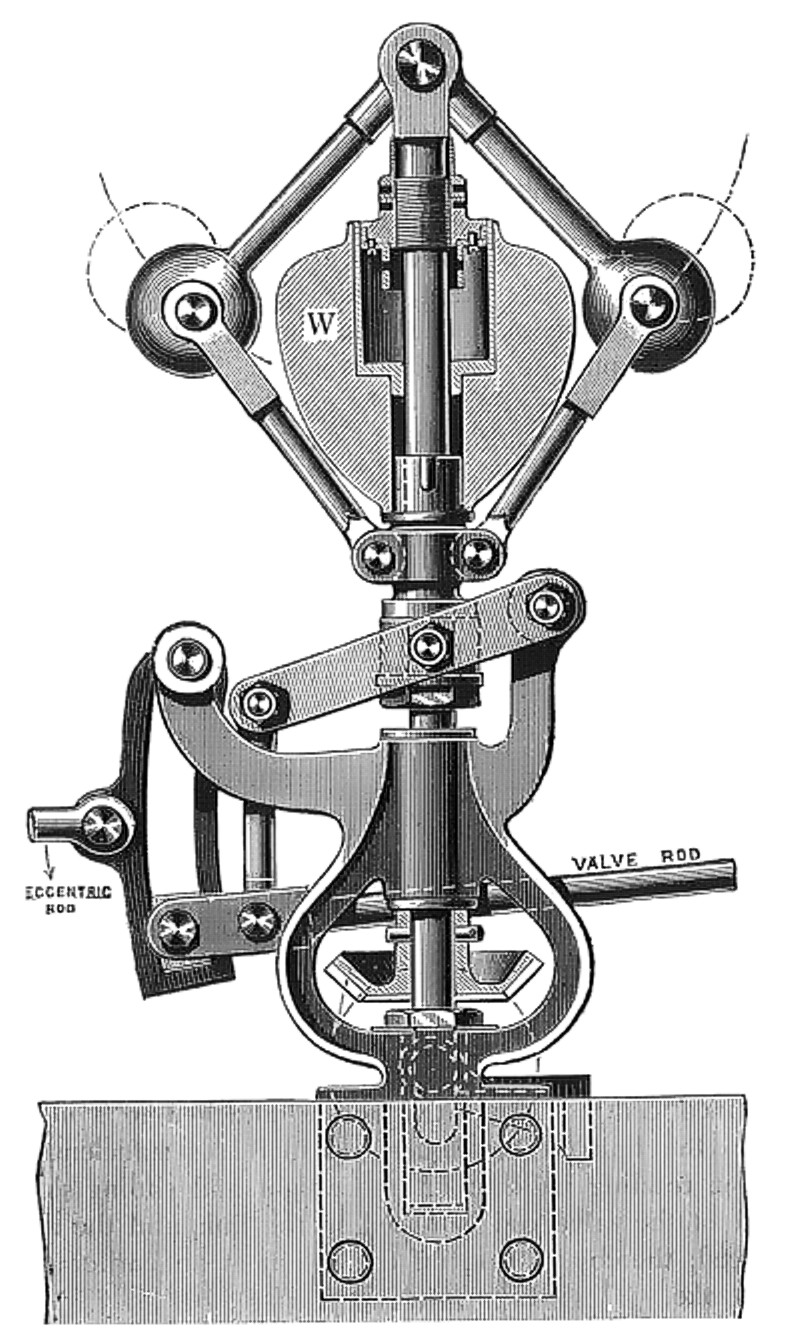
\includegraphics[height=3.4cm]{../../figures/d2_governor.jpg}\\
\credit{Heat Engines (1913), scan by Andy Dingley, Public domain, via Wikimedia Commons}\\[1mm]
\footnotesize\raggedright
Watt's centrifugal governor: a mechanical P controller for steam-engine speed. Maxwell's paper ``On Governors'' (1868) started control theory.
\end{columns}
\end{frame}

% ---------------------------------------------------------------------
\begin{frame}{Worked example: closing a P loop around the robot joint}
\begin{columns}[T]
\column{.47\textwidth}
\centering
\begin{tikzpicture}[node distance=6mm]
  \node[sum] (s1) {};
  \node[blk,right=of s1] (C) {$K_p$};
  \node[blko,right=of C] (G) {$\dfrac{1}{Js^2+Bs}$};
  \draw[sig] ($(s1.west)-(6mm,0)$) node[left,lbl]{$\theta_r$}--(s1);
  \draw[sig] (s1)--(C) node[midway,above,lbl]{$e$};
  \draw[sig] (C)--(G) node[midway,above,lbl]{$T$};
  \draw[sig] (G)--++(12mm,0) node[right,lbl]{$\theta$};
  \fill ($(G.east)+(6mm,0)$) circle (1pt);
  \draw[sig] ($(G.east)+(6mm,0)$)--++(0,-9mm) -| (s1) node[pos=.95,left,lbl]{$-$};
\end{tikzpicture}\\[1mm]
\begin{eqbox}
\[
\frac{\Theta}{\Theta_r}=\frac{K_p}{Js^2+Bs+K_p}
\]
\end{eqbox}
\footnotesize\raggedright
\begin{enumerate}
  \item Compare with $\omega_n^2/(s^2+2\zeta\omega_n s+\omega_n^2)$.
  \item $K_p=50$\,Nm/rad: $\omega_n=\sqrt{K_p/J}=\sqrt{100}=10$\,rad/s.
  \item $\zeta=B/(2\sqrt{K_pJ})=0.1/10=0.01$.
  \item Almost no damping $\Rightarrow$ the arm \hl{rings} for many seconds.
\end{enumerate}
\column{.51\textwidth}
\centering
\begin{tikzpicture}
\begin{axis}[mkplot,width=7.4cm,height=4.6cm,xlabel={time [s]},ylabel={joint angle $\theta$ [rad]},xmin=0,xmax=3,ymin=0,ymax=1.05,
  legend pos=south east]
  \addplot[mkOrange,thick] table[x=t,y=P] {data/joint_pd.dat}; \addlegendentry{P only, $K_p=50$}
  \addplot[mkGray,dashed,domain=0:3] {0.5}; \addlegendentry{target 0.5\,rad}
\end{axis}
\end{tikzpicture}\\
\footnotesize
Feedback alone does not guarantee \hl{good} behaviour: the loop must be designed (sessions 2.5, 2.6).
\end{columns}
\end{frame}

% ---------------------------------------------------------------------
\begin{frame}{Refresher: matrices for state space}
\begin{columns}[T]
\column{.5\textwidth}
\begin{defbox}[Refresher: matrix times vector]
\footnotesize
Each row of $A$ times the vector $\bm x$ gives one entry:
\[
\begin{bmatrix}0&1\\-4&-2\end{bmatrix}\begin{bmatrix}1\\2\end{bmatrix}
=\begin{bmatrix}0\cdot1+1\cdot2\\-4\cdot1-2\cdot2\end{bmatrix}=\begin{bmatrix}2\\-8\end{bmatrix}
\]
\end{defbox}
\small
Why? Two coupled ODEs
\[
\dot x_1=x_2,\qquad \dot x_2=-4x_1-2x_2
\]
fit in one line: $\dot{\bm x}=A\bm x$ with the matrix above.
\column{.48\textwidth}
\small
\textbf{Eigenvalues} = the natural ``speeds'' of $A$:
\begin{eqbox}
\[
\det(\lambda I-A)=0
\]
\end{eqbox}
\footnotesize
\begin{enumerate}
  \item $\lambda I-A=\begin{bmatrix}\lambda&-1\\4&\lambda+2\end{bmatrix}$
  \item $\det=\lambda(\lambda+2)+4=\lambda^2+2\lambda+4$
  \item Roots: $\lambda=-1\pm j1.73$
\end{enumerate}
\hl{Eigenvalues of $A$ = poles of the system.} This is a mass--spring--damper with $m=1$, $k=4$, $c=2$ ($\omega_n=2$, $\zeta=0.5$).
\end{columns}
\end{frame}

% ---------------------------------------------------------------------
\begin{frame}{State-space representation}
\begin{columns}[T]
\column{.48\textwidth}
\small
\term{State} $\bm x$: the few numbers that describe ``where the system is now'' (positions, speeds, currents).
\begin{eqbox}
\[
\dot{\bm x}=A\bm x+B u,\qquad y=C\bm x+D u
\]
\end{eqbox}
\footnotesize
\textbf{Robot joint}, $x_1=\theta$, $x_2=\omega=\dot\theta$, $u=T$:
\[
A=\begin{bmatrix}0&1\\0&-\tfrac BJ\end{bmatrix},\;
B=\begin{bmatrix}0\\ \tfrac1J\end{bmatrix},\;
C=\begin{bmatrix}1&0\end{bmatrix}
\]
\begin{itemize}
  \item Handles many inputs/outputs (a 6-axis arm!); $D=0$ here.
  \item Basis for observers and the Kalman filter (W2D5).
\end{itemize}
\further{$G(s)=C(sI-A)^{-1}B+D$; states are not unique.}
\column{.5\textwidth}
\centering
\begin{tikzpicture}[node distance=5mm,scale=.85,transform shape]
  \node[blk] (B) {$B$};
  \node[sum,right=of B] (s) {};
  \node[blko,right=of s,minimum width=12mm] (I) {$\displaystyle\int$};
  \node[blk,right=of I] (C) {$C$};
  \node[sum,right=of C] (s2) {};
  \node[blk,below=of I] (A) {$A$};
  \node[blk,above=of I] (D) {$D$};
  \draw[sig] ($(B.west)-(7mm,0)$) node[left,lbl]{$u$} -- (B);
  \draw[sig] (B)--(s);
  \draw[sig] (s)--(I) node[midway,above,lbl]{$\dot{\bm x}$};
  \draw[sig] (I)--(C) node[midway,above,lbl]{$\bm x$};
  \draw[sig] (C)--(s2);
  \draw[sig] (s2)--++(8mm,0) node[right,lbl]{$y$};
  \draw[sig] ($(I.east)+(3mm,0)$) |- (A);
  \draw[sig] (A) -| (s);
  \draw[sig] ($(B.west)-(3mm,0)$) |- (D);
  \draw[sig] (D) -| (s2);
  \fill ($(I.east)+(3mm,0)$) circle (1pt); \fill ($(B.west)-(3mm,0)$) circle (1pt);
\end{tikzpicture}\\[3mm]
\begin{notebox}
One integrator per state variable: integrators ``remember'' the state. Eigenvalues of the joint's $A$: $0$ and $-B/J=-0.2$\,s$^{-1}$ (the same as the poles of $1/(Js^2+Bs)$).
\end{notebox}
\end{columns}
\end{frame}

% ---------------------------------------------------------------------
\begin{frame}{The joint motor in both representations}
\begin{columns}[T]
\column{.44\textwidth}
\centering
\begin{circuitikz}[scale=.78,transform shape,font=\small]
  \draw (0,0) to[V,v<=$v_a$] (0,2.6)
        to[R=$R$,i>^=$i_a$] (2.6,2.6)
        to[L=$L_a$] (4.6,2.6)
        to[short] (4.6,2.2);
  \draw (4.6,0.4) to[short] (4.6,0) -- (0,0);
  \draw[thick,fill=mkPale] (4.6,1.3) circle (.75);
  \node at (4.6,1.3) {M};
  \node[anchor=west] at (5.4,2.0) {$e=k_e\omega$};
  \node[font=\small] at (4.6,2.38) {$+$};
  \node[font=\small] at (4.6,0.22) {$-$};
  \draw[very thick,mkBlue] (5.35,1.3)--(6.6,1.3);
  \draw[thick,fill=mkCream] (6.6,0.7) rectangle (7.0,1.9);
  \node[anchor=north,align=center,font=\footnotesize] at (6.8,0.6) {$J,B$};
  \draw[-{Latex},mkOrange,thick] (5.8,1.75) arc (120:60:.5) node[right]{$\omega$};
\end{circuitikz}\\[2mm]
\footnotesize
\begin{align*}
L_a\tfrac{di_a}{dt}&=v_a-Ri_a-k_e\,\omega\quad\text{(KVL)}\\
J\tfrac{d\omega}{dt}&=k_t\,i_a-B\omega\quad\text{(Newton)}
\end{align*}
SI units: $k_t$ [Nm/A] $=k_e$ [V\,s/rad].
\column{.54\textwidth}
\footnotesize
\textbf{State space}: two energy stores $\Rightarrow$ two states $\bm x=[i_a,\ \omega]^{\!\top}$, $u=v_a$, $y=\omega$:
\[
A=\begin{bmatrix}-\frac{R}{L_a}&-\frac{k_e}{L_a}\\[2pt]\frac{k_t}{J}&-\frac{B}{J}\end{bmatrix},\;
B=\begin{bmatrix}\frac1{L_a}\\[2pt]0\end{bmatrix},\;
C=\begin{bmatrix}0&1\end{bmatrix}
\]
\textbf{Transfer function} (Laplace of both equations, eliminate $I_a$):
\begin{eqbox}
\[
\frac{\Omega(s)}{V_a(s)}=\frac{k_t}{(L_as+R)(Js+B)+k_tk_e}
\]
\end{eqbox}
\begin{itemize}
  \item The $k_tk_e$ term is \term{back-EMF}: the motor has a \hl{built-in feedback loop} (faster $\Rightarrow$ less current).
  \item Load torque $T_L$ (gravity, payload) is a second input: a disturbance.
\end{itemize}
\end{columns}
\end{frame}

% ---------------------------------------------------------------------
\begin{frame}{Worked example: a small joint servo motor}
\begin{columns}[T]
\column{.45\textwidth}
\footnotesize
Motor: $R=1.2\,\Omega$, $L_a=2.4$\,mH, $k_t=k_e=0.1$\,Nm/A, $J=2\times10^{-4}$\,kg\,m$^2$ (motor + reflected link), $B=10^{-5}$\,Nm\,s/rad.
\begin{enumerate}
  \item Denominator divided by $L_aJ$:
  \[s^2+500\,s+20\,860\]
  \item Eigenvalues/poles: $-46$\,s$^{-1}$ (mechanical, slow), $-454$\,s$^{-1}$ (electrical, fast).
  \item DC gain: $G(0)=\dfrac{k_t}{RB+k_tk_e}\approx10$\,rad/s per V.
  \item 24\,V step $\Rightarrow$ $\approx240$\,rad/s (2290\,rpm), settles in $\approx4/46=87$\,ms.
\end{enumerate}
Starting current $\approx24\,\mathrm{V}/1.2\,\Omega=20$\,A: a reason for current control (W1D5).
\column{.53\textwidth}
\centering
\begin{tikzpicture}
\begin{groupplot}[group style={group size=1 by 2,vertical sep=3mm,x descriptions at=edge bottom},
  mkplot,width=7.4cm,height=3.6cm,xmin=0,xmax=150]
\nextgroupplot[ylabel={$\omega$ [rad/s]},ymin=0,ymax=260,legend pos=south east]
  \addplot[mkBlue,very thick] table[x=t,y=w] {data/dcmotor_step.dat}; \addlegendentry{second-order model}
  \addplot[mkSky,thick,dashed] table[x=t,y=wapprox] {data/dcmotor_step.dat}; \addlegendentry{$L_a\rightarrow0$ approx.}
\nextgroupplot[ylabel={$i_a$ [A]},xlabel={time [ms]},ymin=0,ymax=20]
  \addplot[mkOrange,thick] table[x=t,y=i] {data/dcmotor_step.dat};
\end{groupplot}
\end{tikzpicture}\\
\footnotesize 24\,V voltage step, no load; simulated from the state-space model.
\end{columns}
\end{frame}

% ---------------------------------------------------------------------
\begin{frame}{Session 2.3 -- Check your understanding}
\begin{columns}[T]
\column{.6\textwidth}
\begin{keybox}[Check your understanding]
\begin{enumerate}
  \item Reduce the loop on the right to one transfer function $Y/R$ for $C=4$ and $G=\frac{1}{s+1}$. What is the final value for a unit step?
  \item In the P-controlled joint, what happens to $\omega_n$ and $\zeta$ if the payload doubles $J$?
  \item How many state variables does the DC motor have, and why?
\end{enumerate}
\end{keybox}
\column{.37\textwidth}
\centering
\begin{tikzpicture}[node distance=5mm]
  \node[sum] (s1) {};
  \node[blk,right=of s1] (C) {$C$};
  \node[blko,right=of C] (G) {$G$};
  \draw[sig] ($(s1.west)-(5mm,0)$) node[left,lbl]{$r$}--(s1);
  \draw[sig] (s1)--(C); \draw[sig] (C)--(G);
  \draw[sig] (G)--++(10mm,0) node[right,lbl]{$y$};
  \fill ($(G.east)+(5mm,0)$) circle (1pt);
  \draw[sig] ($(G.east)+(5mm,0)$)--++(0,-8mm) -| (s1) node[pos=.95,left,lbl]{$-$};
\end{tikzpicture}
\end{columns}
\end{frame}

% ---------------------------------------------------------------------
\begin{frame}{Session 2.3 -- Summary and key terms}
\begin{columns}[T]
\column{.55\textwidth}
\begin{keybox}[Key take-aways]
\footnotesize
\begin{itemize}
  \item Feedback = measure, compare, correct; it fights unknown disturbances.
  \item Block diagrams: series multiply, parallel add, feedback gives $G_1/(1+G_1G_2)$.
  \item $S=1/(1+L)$ and $T=L/(1+L)$ describe every feedback loop.
  \item State space $\dot{\bm x}=A\bm x+Bu$: eigenvalues of $A$ = poles.
  \item P control of an inertia gives an \hl{undamped} spring: we need more (D).
\end{itemize}
\end{keybox}
\column{.42\textwidth}
\begin{defbox}[Key terms]
\footnotesize
\term{Open / closed loop}: without / with measurement.\\
\term{Summing junction}: adds or subtracts signals.\\
\term{Loop gain} $L=CG$: gain once around.\\
\term{Sensitivity} $S$: fraction of disturbance left.\\
\term{State}: variables that store energy/memory.
\end{defbox}
\end{columns}
\end{frame}

% =====================================================================
\section{2.4 Frequency Response and Bode Plots}
% =====================================================================

\begin{frame}{Refresher: what a sinusoidal frequency response means}
\begin{columns}[T]
\column{.48\textwidth}
\centering
\begin{tikzpicture}
\begin{axis}[mkplot,width=7.0cm,height=4.0cm,xmin=0,xmax=2,ymin=-1.25,ymax=1.25,xlabel={time (periods)},ytick={-1,0,1},
  legend style={at={(0.5,1.02)},anchor=south},legend columns=2]
  \addplot[mkBlue,thick,domain=0:2,samples=120] {sin(360*x)}; \addlegendentry{input $u$}
  \addplot[mkOrange,very thick,domain=0:2,samples=120] {0.6*sin(360*x-60)}; \addlegendentry{output $y$}
  \draw[mkNavy,<->] (axis cs:0.25,0)--(axis cs:0.25,1) node[pos=.5,left,font=\tiny]{$\hat u$};
  \draw[mkOrange,<->] (axis cs:1.42,0)--(axis cs:1.42,0.6) node[pos=.5,right,font=\tiny]{$\hat y$};
  \draw[mkGray,<->] (axis cs:1.25,1.05)--(axis cs:1.4167,1.05) node[midway,above,font=\tiny]{lag};
\end{axis}
\end{tikzpicture}\\[1mm]
\footnotesize\raggedright Wave a robot arm slowly: the tip follows. Wave it fast: the tip moves less and \hl{lags behind}.
\column{.5\textwidth}
\begin{defbox}[Refresher: frequency response]
\footnotesize
A linear stable system driven by a sine answers with a sine of the \hl{same frequency}, only scaled and shifted.
\end{defbox}
\begin{eqbox}
\[
y=|G(j\omega)|\,\hat u\,\sin\!\big(\omega t+\angle G(j\omega)\big)
\]
\end{eqbox}
\footnotesize
for input $u=\hat u\sin\omega t$. \textbf{Recipe}: replace $s$ by $j\omega$.\\
Example $G=\dfrac{1}{s+1}$:
\begin{enumerate}
  \item $\omega=1$\,rad/s: $G(j1)=\dfrac{1}{1+j}=0.707\angle-45^\circ$
  \item $\omega=10$\,rad/s: $\dfrac{1}{1+10j}=0.0995\angle-84^\circ$
\end{enumerate}
Faster input $\Rightarrow$ smaller output and more lag.
\end{columns}
\end{frame}

% ---------------------------------------------------------------------
\begin{frame}{Refresher: decibels and logarithmic scales}
\begin{columns}[T]
\column{.42\textwidth}
\begin{defbox}[Refresher: the decibel]
\footnotesize
Gains span from 0.001 to 1000: a \hl{log scale} keeps both visible. Gain in decibels:
\end{defbox}
\begin{eqbox}
\[
|G|_{\mathrm{dB}}=20\log_{10}|G|
\]
\end{eqbox}
\footnotesize
\begin{itemize}
  \item Gains in series multiply $\Rightarrow$ their dB values \hl{add}.
  \item $-3$\,dB $=0.707$: the usual edge of the ``bandwidth''.
  \item A \term{decade} = frequency $\times10$.
\end{itemize}
\column{.25\textwidth}
\centering
\footnotesize
\begin{tabular}{@{}rr@{}}
\toprule
$|G|$ & dB\\
\midrule
1000 & $+60$\\
100 & $+40$\\
10 & $+20$\\
2 & $+6$\\
1 & $0$\\
0.707 & $-3$\\
0.5 & $-6$\\
0.1 & $-20$\\
0.01 & $-40$\\
\bottomrule
\end{tabular}
\column{.3\textwidth}
\centering
\begin{tikzpicture}[font=\scriptsize]
  \draw[thick,mkNavy] (0,0)--(4,0);
  \foreach \x/\l in {0/0.1,1/1,2/10,3/100,4/1000}{\draw[thick,mkNavy] (\x,-.1)--(\x,.1); \node[below] at (\x,-.1){\l};}
  \foreach \d in {0,1,2,3}{\foreach \m in {2,3,4,5,6,7,8,9}{\draw[mkGray] ({\d+log10(\m)},-.05)--({\d+log10(\m)},.05);}}
  \draw[mkOrange,<->] (1,.3)--(2,.3) node[midway,above]{1 decade};
  \node[mkGray] at (2,-.75) {$\omega$ [rad/s], log axis};
\end{tikzpicture}\\[4mm]
\footnotesize\raggedright
Equal steps on the axis = equal \emph{ratios}.\\[2pt]
Example: $|G|=0.05$ $\Rightarrow$ $20\log_{10}0.05=-26$\,dB.
\end{columns}
\end{frame}

% ---------------------------------------------------------------------
\begin{frame}{How to read a Bode plot}
\begin{columns}[T]
\column{.42\textwidth}
\footnotesize
A \term{Bode plot} = frequency response for all $\omega$: magnitude in dB (top) and phase in degrees (bottom), both over a log frequency axis.\\[1mm]
\textbf{Reading it}:
\begin{enumerate}
  \item pick $\omega$ (e.g.\ 0.1\,rad/s)
  \item read magnitude: 40\,dB $\Rightarrow$ gain $\times100$
  \item read phase: $\approx-85^\circ$ (output lags)
\end{enumerate}
\textbf{Straight-line rules}:
\begin{itemize}
  \item each pole: $-20$\,dB/decade after its corner, phase drops by $90^\circ$
  \item each zero: $+20$\,dB/decade, phase rises by $90^\circ$
  \item integrator $1/s$: $-20$\,dB/decade, $-90^\circ$ everywhere
\end{itemize}
\begin{minipage}{.11\linewidth}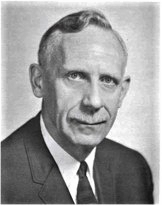
\includegraphics[width=\linewidth]{../../figures/d2_bode_portrait.png}\end{minipage}\hfill
\begin{minipage}{.82\linewidth}\tiny H.\,W.\ Bode (1905--1982), Bell Labs. \credit{Unknown author, Public domain, via Wikimedia Commons}\end{minipage}
\column{.56\textwidth}
\centering
\begin{tikzpicture}
\begin{groupplot}[group style={group size=1 by 2,vertical sep=4mm,x descriptions at=edge bottom},
  mkplot,width=7.6cm,height=3.3cm,xmode=log,xmin=0.01,xmax=1000,log basis x=10]
\nextgroupplot[ylabel={$|G|$ [dB]},ymin=-30,ymax=70,ytick={-20,0,20,40,60},legend pos=north east,
  title={\scriptsize $G(s)=\dfrac{100(s+1)}{s(s+10)}$},title style={yshift=-1mm}]
  \addplot[mkBlue,very thick,domain=-2:3,samples=150] ({10^x},{20*log10(100)+10*log10(1+10^(2*x))-20*x-10*log10(100+10^(2*x))});
  \addlegendentry{exact}
  \addplot[mkOrange,thick,dashed] coordinates {(0.01,60)(1,20)(10,20)(1000,-20)}; \addlegendentry{straight lines}
  \fill[mkRed] (axis cs:0.1,40) circle (2pt);
\nextgroupplot[ylabel={$\angle G$ [deg]},xlabel={$\omega$ [rad/s]},ymin=-100,ymax=0,ytick={-90,-45,0}]
  \addplot[mkBlue,very thick,domain=-2:3,samples=150] ({10^x},{-90+atan(10^x)-atan(10^x/10)});
  \addplot[mkOrange,thick,dashed] coordinates {(0.01,-90)(0.1,-90)(1,-45)(10,-45)(100,-90)(1000,-90)};
\end{groupplot}
\end{tikzpicture}\\
\footnotesize Integrator: $-20$\,dB/dec; zero at 1 flattens; pole at 10 bends down again.
\end{columns}
\end{frame}

% ---------------------------------------------------------------------
\begin{frame}{Worked example: Bode plot of a first-order lag}
\begin{columns}[T]
\column{.55\textwidth}
\centering
\begin{tikzpicture}
\begin{groupplot}[group style={group size=1 by 2,vertical sep=4mm,x descriptions at=edge bottom},
  mkplot,width=8.0cm,height=3.7cm,xmode=log,xmin=0.2,xmax=2000]
\nextgroupplot[ylabel={$|G|$ [dB]},ymin=-42,ymax=6,ytick={-40,-20,-3,0},legend pos=south west]
  \addplot[mkBlue,very thick,domain=-0.7:3.3,samples=120] ({10^x},{-10*log10(1+(10^x/20)^2)}); \addlegendentry{exact}
  \addplot[mkOrange,thick,dashed] coordinates {(0.2,0)(20,0)(2000,-40)}; \addlegendentry{asymptotes}
  \addplot[only marks,mark=*,mark size=1.8pt,mkRed] coordinates {(2,-0.04)(20,-3)(200,-20)};
\nextgroupplot[ylabel={$\angle G$ [deg]},xlabel={$\omega$ [rad/s]},ymin=-95,ymax=5,ytick={-90,-45,0}]
  \addplot[mkBlue,very thick,domain=-0.7:3.3,samples=120] ({10^x},{-atan(10^x/20)});
  \addplot[only marks,mark=*,mark size=1.8pt,mkRed] coordinates {(2,-5.7)(20,-45)(200,-84.3)};
\end{groupplot}
\end{tikzpicture}
\column{.43\textwidth}
\small
Current-controlled joint motor seen from the speed command, $\tau=0.05$\,s:
\begin{eqbox}
\[
G(s)=\frac{1}{\tau s+1},\quad \omega_b=\frac1\tau=20\ \mathrm{rad/s}
\]
\end{eqbox}
\footnotesize
\begin{enumerate}
  \item $\omega=2$: $|G|=1/\sqrt{1+0.01}=0.995$ ($-0.04$\,dB), $-5.7^\circ$.
  \item $\omega=20$ (corner): $1/\sqrt2=0.707$ ($-3$\,dB), $-45^\circ$.
  \item $\omega=200$: $\approx0.1$ ($-20$\,dB), $-84^\circ$.
\end{enumerate}
\hl{Two straight lines} (flat, then $-20$\,dB/dec) are within 3\,dB everywhere.
\end{columns}
\end{frame}

% ---------------------------------------------------------------------
\begin{frame}{Resonance: pushing a swing at the right moment}
\begin{columns}[T]
\column{.57\textwidth}
\centering
\begin{tikzpicture}
\begin{groupplot}[group style={group size=1 by 2,vertical sep=4mm,x descriptions at=edge bottom},
  mkplot,width=8.0cm,height=3.9cm,xmode=log,xmin=0.1,xmax=10,
  cycle list={{mkRed,thick},{mkOrange,thick},{mkBlue,very thick},{mkMid,thick,dashed},{mkSky,thick,dotted}}]
\nextgroupplot[ylabel={$|G|$ [dB]},ymin=-40,ymax=22,legend pos=south west,legend columns=2]
  \addplot+[domain=-1:1,samples=300] ({10^x},{-10*log10((1-10^(2*x))^2+(2*0.05*10^x)^2)}); \addlegendentry{$\zeta=0.05$}
  \addplot+[domain=-1:1,samples=200] ({10^x},{-10*log10((1-10^(2*x))^2+(2*0.2*10^x)^2)}); \addlegendentry{$0.2$}
  \addplot+[domain=-1:1,samples=200] ({10^x},{-10*log10((1-10^(2*x))^2+(2*0.5*10^x)^2)}); \addlegendentry{$0.5$}
  \addplot+[domain=-1:1,samples=200] ({10^x},{-10*log10((1-10^(2*x))^2+(2*0.707*10^x)^2)}); \addlegendentry{$0.707$}
  \addplot+[domain=-1:1,samples=200] ({10^x},{-10*log10((1-10^(2*x))^2+(2*1*10^x)^2)}); \addlegendentry{$1$}
\nextgroupplot[ylabel={$\angle G$ [deg]},xlabel={$\omega/\omega_n$},ymin=-185,ymax=5,ytick={-180,-90,0}]
  \addplot+[domain=-1:1,samples=300] ({10^x},{-atan2(2*0.05*10^x,1-10^(2*x))});
  \addplot+[domain=-1:1,samples=200] ({10^x},{-atan2(2*0.2*10^x,1-10^(2*x))});
  \addplot+[domain=-1:1,samples=200] ({10^x},{-atan2(2*0.5*10^x,1-10^(2*x))});
  \addplot+[domain=-1:1,samples=200] ({10^x},{-atan2(2*0.707*10^x,1-10^(2*x))});
  \addplot+[domain=-1:1,samples=200] ({10^x},{-atan2(2*1*10^x,1-10^(2*x))});
\end{groupplot}
\end{tikzpicture}
\column{.41\textwidth}
\small
Small pushes at the swing's own rhythm give a \hl{big} motion: that is \term{resonance}.
\begin{eqbox}
\[
|G(j\omega_n)|=\frac{1}{2\zeta}
\]
\end{eqbox}
\footnotesize
\begin{itemize}
  \item Below $\omega_n$: output follows ($0$\,dB, $0^\circ$).
  \item At $\omega_n$: peak, phase $-90^\circ$.
  \item Above $\omega_n$: falls with $-40$\,dB/decade, phase $\rightarrow-180^\circ$.
  \item $\zeta=0.05$: peak $1/0.1=10$ ($+20$\,dB) -- typical of a \hl{gearbox or belt} resonance in a robot joint.
\end{itemize}
\further{peak $M_r=1/(2\zeta\sqrt{1-\zeta^2})$ at $\omega_n\sqrt{1-2\zeta^2}$.}
\end{columns}
\end{frame}

% ---------------------------------------------------------------------
\begin{frame}{Measuring a frequency response on a robot axis}
\begin{columns}[T]
\column{.48\textwidth}
\centering
\begin{tikzpicture}
\begin{groupplot}[group style={group size=1 by 3,vertical sep=2.5mm,x descriptions at=edge bottom},
  mkplot,width=7.0cm,height=2.55cm,xmin=0,xmax=1,ymin=-1.4,ymax=1.4,ytick={-1,0,1},
  every axis title/.style={at={(0.01,0.98)},anchor=north west,font=\tiny\bfseries,fill=white,inner sep=1pt}]
\nextgroupplot[title={chirp (sweep) 1$\rightarrow$40\,Hz}]
  \addplot[mkBlue,thin] table[x=t,y=chirp] {data/excitation.dat};
\nextgroupplot[title={PRBS (random-looking binary)}]
  \addplot[mkOrange,thin,const plot] table[x=t,y=prbs] {data/excitation.dat};
\nextgroupplot[title={stepped sine (3, 6, 12, 24\,Hz)},xlabel={time [s]}]
  \addplot[mkMid,thin] table[x=t,y=stepped] {data/excitation.dat};
\end{groupplot}
\end{tikzpicture}
\column{.5\textwidth}
\centering
\begin{tikzpicture}[node distance=5mm,scale=.9,transform shape]
  \node[sum] (s1) {};
  \node[blk,right=of s1] (C) {$C(s)$\\controller};
  \node[sum,right=6mm of C] (s2) {};
  \node[blk,right=of s2] (G) {$G(s)$\\drive+joint};
  \draw[sig] ($(s1.west)-(5mm,0)$) node[left,lbl]{$r$}--(s1);
  \draw[sig] (s1)--(C);
  \draw[sig] (C)--(s2);
  \draw[sig] (s2)--(G) node[midway,above,lbl]{$u$};
  \draw[sig] (G)--++(12mm,0) node[right,lbl]{$y$};
  \fill ($(G.east)+(6mm,0)$) circle (1pt);
  \draw[sig] ($(G.east)+(6mm,0)$)--++(0,-11mm) -| (s1) node[pos=.95,left,lbl]{$-$};
  \node[blko,above=5mm of s2,minimum width=14mm] (inj) {test signal $w$};
  \draw[sig,mkOrange] (inj)--(s2);
\end{tikzpicture}\\[1mm]
\footnotesize\raggedright
\begin{itemize}
  \item The drive \hl{adds} a test signal $w$ while the joint is held in closed loop (safe against gravity).
  \item It records $u$ and $y$ and computes $|G|$ and $\angle G$ at each frequency.
  \item Amplitude: big enough to beat friction and noise, small enough to stay within limits.
  \item Average several runs to reduce noise.
\end{itemize}
\further{FRF $\hat G=\hat S_{wy}/\hat S_{wu}$ from cross-spectra.}
\end{columns}
\end{frame}

% ---------------------------------------------------------------------
\begin{frame}{Measured response of a compliant joint: two masses and a spring}
\begin{columns}[T]
\column{.55\textwidth}
\centering
\begin{tikzpicture}
\begin{groupplot}[group style={group size=1 by 2,vertical sep=4mm,x descriptions at=edge bottom},
  mkplot,width=8.0cm,height=3.7cm,xmode=log,xmin=1,xmax=1000]
\nextgroupplot[ylabel={$|\Omega_m/T_m|$ [dB]},ymin=-50,ymax=50,legend pos=south west]
  \addplot[mkBlue,very thick] table[x=f,y=mag] {data/twomass.dat}; \addlegendentry{two-mass (real)}
  \addplot[mkOrange,thick,dashed] table[x=f,y=magrigid] {data/twomass.dat}; \addlegendentry{rigid model $1/((J_m+J_l)s)$}
  \node[font=\tiny,anchor=north] at (axis cs:130,-22) {anti-res.};
  \node[font=\tiny,anchor=south] at (axis cs:260,30) {res.};
\nextgroupplot[ylabel={coherence $\gamma^2$},xlabel={frequency [Hz]},ymin=0,ymax=1.1,ytick={0,0.5,1}]
  \addplot[mkMid,very thick] table[x=f,y=coh] {data/twomass.dat};
\end{groupplot}
\end{tikzpicture}
\column{.43\textwidth}
\footnotesize
Motor $J_m=2\times10^{-4}$ and load $J_l=6\times10^{-4}$\,kg\,m$^2$ joined by a springy gear/shaft $k=400$\,Nm/rad:
\begin{eqbox}
\[
f_r=\frac{1}{2\pi}\sqrt{k\,\frac{J_m+J_l}{J_mJ_l}}=260\ \mathrm{Hz}
\]
\end{eqbox}
\begin{itemize}
  \item Up to $\approx$\,50\,Hz the rigid model fits; near 130--260\,Hz it is \hl{completely wrong}.
  \item \term{Coherence} $\gamma^2$ (0\ldots1): trust the measurement only where $\gamma^2\gtrsim0.8$.
  \item Rule: keep the control bandwidth \hl{below the first resonance} (notch filters: W1D4).
\end{itemize}
\end{columns}
\end{frame}

% ---------------------------------------------------------------------
\begin{frame}{Session 2.4 -- Check your understanding}
\begin{columns}[T]
\column{.62\textwidth}
\begin{keybox}[Check your understanding]
\begin{enumerate}
  \item Convert a gain of $0.1$ and a gain of $1000$ to dB.
  \item At 10\,Hz a 1\,V input sine gives a 2\,V output sine that lags by a quarter period. What are $|G|$ in dB and $\angle G$?
  \item A robot joint with a strain-wave gear (right) shows a sharp peak at 40\,Hz in its Bode plot. What does this mean for the controller?
\end{enumerate}
\end{keybox}
\column{.35\textwidth}
\centering
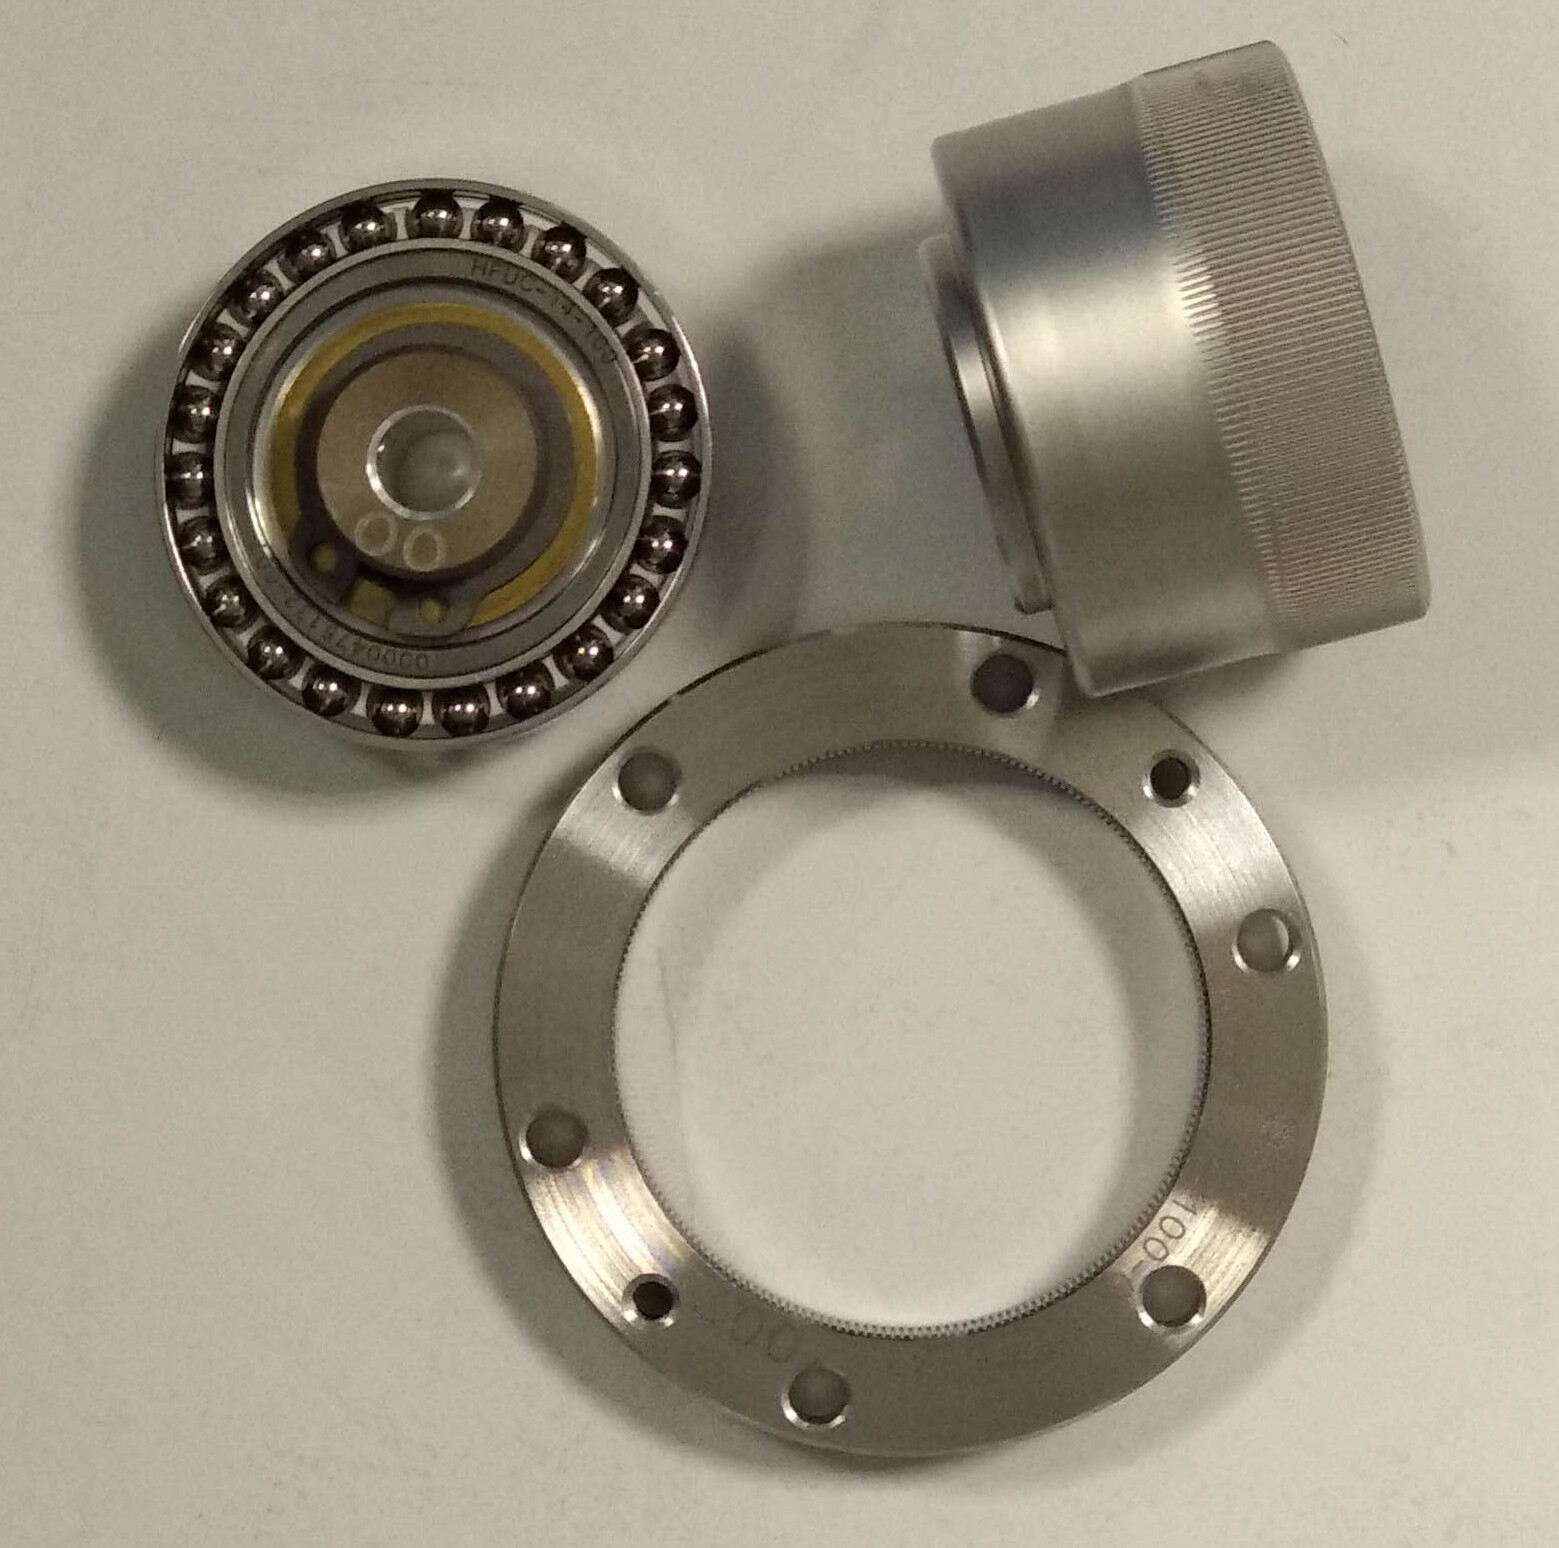
\includegraphics[height=3.6cm]{../../figures/d2_harmonic_drive.jpg}\\
\credit{Pieceofmetalwork, CC BY-SA 4.0, via Wikimedia Commons}\\
\footnotesize Strain-wave (harmonic) gear set: light, zero backlash, but \hl{springy}.
\end{columns}
\end{frame}

% ---------------------------------------------------------------------
\begin{frame}{Session 2.4 -- Summary and key terms}
\begin{columns}[T]
\column{.55\textwidth}
\begin{keybox}[Key take-aways]
\footnotesize
\begin{itemize}
  \item Sine in $\Rightarrow$ sine out: gain $|G(j\omega)|$ and phase $\angle G(j\omega)$.
  \item Bode plot: dB and degrees over log frequency.
  \item Each pole: $-20$\,dB/dec and up to $-90^\circ$; corner at $\omega=1/\tau$ is $-3$\,dB.
  \item Low $\zeta$ $\Rightarrow$ sharp resonance peak $1/(2\zeta)$.
  \item Measured Bode plots reveal joint resonances $\Rightarrow$ \hl{limit the bandwidth}.
\end{itemize}
\end{keybox}
\column{.42\textwidth}
\begin{defbox}[Key terms]
\footnotesize
\term{Frequency response}: gain and phase vs.\ frequency.\\
\term{Decibel}: $20\log_{10}$ of a gain.\\
\term{Corner frequency}: where asymptotes meet.\\
\term{Resonance}: large response near $\omega_n$.\\
\term{Coherence}: measurement quality, 0\ldots1.
\end{defbox}
\end{columns}
\end{frame}

% =====================================================================
\section{2.5 PID Control}
% =====================================================================

\begin{frame}{P, I and D: present, past and future of the error}
\begin{columns}[T]
\column{.5\textwidth}
\centering
\begin{tikzpicture}
\begin{axis}[mkplot,width=6.9cm,height=4.4cm,xlabel={time [s]},ylabel={$y$},xmin=0,xmax=20,ymin=0,ymax=1.6,
  title={\scriptsize P only, $G=1/(s+1)^3$},title style={yshift=-1.5mm},legend pos=north east,legend columns=2]
  \addplot[mkSky,thick] table[x=t,y=k05] {data/p_control.dat}; \addlegendentry{$K_p=0.5$}
  \addplot[mkMid,thick] table[x=t,y=k1] {data/p_control.dat}; \addlegendentry{$1$}
  \addplot[mkBlue,very thick] table[x=t,y=k2] {data/p_control.dat}; \addlegendentry{$2$}
  \addplot[mkOrange,thick] table[x=t,y=k4] {data/p_control.dat}; \addlegendentry{$4$}
\end{axis}
\end{tikzpicture}
\column{.5\textwidth}
\centering
\begin{tikzpicture}
\begin{axis}[mkplot,width=6.9cm,height=4.4cm,xlabel={time [s]},xmin=0,xmax=20,ymin=0,ymax=1.6,
  title={\scriptsize same plant, four controllers},title style={yshift=-1.5mm},legend pos=north east,legend columns=2]
  \addplot[mkSky,thick] table[x=t,y=P] {data/pid_compare.dat}; \addlegendentry{P}
  \addplot[mkMid,thick,dashed] table[x=t,y=PD] {data/pid_compare.dat}; \addlegendentry{PD}
  \addplot[mkOrange,thick] table[x=t,y=PI] {data/pid_compare.dat}; \addlegendentry{PI}
  \addplot[mkBlue,very thick] table[x=t,y=PID] {data/pid_compare.dat}; \addlegendentry{PID}
\end{axis}
\end{tikzpicture}
\end{columns}
\begin{columns}[T]
\column{.42\textwidth}
\begin{eqbox}
\footnotesize
\[
u(t)=K_p\,e+K_i\!\int_0^t\!e\,d\tau+K_d\,\dot e
\]
\end{eqbox}
\footnotesize
\textbf{P} = now, \textbf{I} = accumulated past, \textbf{D} = trend (future).
\column{.56\textwidth}
\footnotesize
\begin{tabular}{@{}llll@{}}
\toprule
More \ldots & speed & overshoot & steady-state error\\
\midrule
P ($K_p$) & faster & larger & smaller, not zero\\
I ($K_i$) & faster & larger & \hl{removed}\\
D ($K_d$) & similar & smaller & no effect (noise $\uparrow$)\\
\bottomrule
\end{tabular}
\end{columns}
\end{frame}

% ---------------------------------------------------------------------
\begin{frame}{PD control of a joint = a virtual spring and damper}
\begin{columns}[T]
\column{.45\textwidth}
\centering
\begin{tikzpicture}[font=\scriptsize]
  % wall / target
  \fill[pattern=north east lines,pattern color=mkGray] (-0.3,-1.2) rectangle (0,1.2);
  \draw[thick] (0,-1.2)--(0,1.2);
  % spring
  \draw[thick,mkBlue,decorate,decoration={zigzag,amplitude=2.5mm,segment length=3mm}] (0,.6)--(2.4,.6);
  \node[mkBlue,above] at (1.2,.9) {$K_p$ (spring)};
  % damper
  \draw[thick,mkOrange] (0,-.6)--(1.0,-.6); \draw[thick,mkOrange] (1.0,-.85) rectangle (1.6,-.35);
  \draw[thick,mkOrange] (1.25,-.6)--(2.4,-.6); \draw[thick,mkOrange] (1.25,-.8)--(1.25,-.4);
  \node[mkOrange,below] at (1.3,-.9) {$K_d$ (damper)};
  % mass
  \draw[thick,fill=mkPale,draw=mkNavy] (2.4,-1.0) rectangle (3.6,1.0); \node at (3.0,0) {$J$};
  \draw[-{Latex},thick,mkNavy] (3.0,1.25)--(3.9,1.25) node[right]{$\theta$};
  \node[mkGray,align=center] at (1.6,-1.6) {spring anchored at the target $\theta_r$};
\end{tikzpicture}\\[2mm]
\begin{eqbox}
\[
T=K_p(\theta_r-\theta)-K_d\,\dot\theta
\]
\end{eqbox}
\footnotesize D acts on the measured speed $\dot\theta$ (no kick on target jumps).
\column{.52\textwidth}
\small
The controller makes the joint \hl{feel} like a mass on a spring with a shock absorber -- the car suspension from W1D2.
\begin{defbox}[Worked example: choose the gains]
\footnotesize
Target: $\omega_n=10$\,rad/s, $\zeta=0.7$; joint $J=0.5$, $B=0.1$.
\begin{enumerate}
  \item Stiffness: $K_p=J\omega_n^2=0.5\cdot100=50$\,Nm/rad.
  \item Total damping $2\zeta\omega_nJ=2\cdot0.7\cdot10\cdot0.5=7$\,Nm\,s/rad.
  \item $K_d=7-B=6.9\approx7$\,Nm\,s/rad.
  \item Expect $\approx5$\,\% overshoot, settling $4/(\zeta\omega_n)\approx0.6$\,s.
\end{enumerate}
\end{defbox}
\end{columns}
\end{frame}

% ---------------------------------------------------------------------
\begin{frame}{Effect of D on the joint: from ringing to smooth}
\begin{columns}[T]
\column{.56\textwidth}
\centering
\begin{tikzpicture}
\begin{axis}[mkplot,width=8.0cm,height=5.4cm,xlabel={time [s]},ylabel={joint angle $\theta$ [rad]},xmin=0,xmax=3,ymin=0,ymax=1.05,
  legend pos=north east,legend cell align=left]
  \addplot[mkSky,thick] table[x=t,y=P] {data/joint_pd.dat}; \addlegendentry{P, $K_d=0$ ($\zeta=0.01$)}
  \addplot[mkOrange,thick,dashed] table[x=t,y=PDlow] {data/joint_pd.dat}; \addlegendentry{PD, $K_d=3$ ($\zeta=0.31$)}
  \addplot[mkBlue,very thick] table[x=t,y=PD] {data/joint_pd.dat}; \addlegendentry{PD, $K_d=7$ ($\zeta=0.71$)}
  \addplot[mkGray,dashed,domain=0:3] {0.5};
\end{axis}
\end{tikzpicture}\\
\footnotesize Step of 0.5\,rad, $K_p=50$\,Nm/rad, simulated.
\column{.42\textwidth}
\small
\begin{itemize}
  \item Same $K_p$ $\Rightarrow$ same stiffness and roughly same speed.
  \item $K_d$ only adds \hl{damping}: overshoot falls from 97\,\% to 4\,\%.
  \item Too much $K_d$: sluggish, and it amplifies encoder noise.
\end{itemize}
\begin{notebox}
\footnotesize In a servo drive, the D-term on position is often realised by the \hl{inner velocity loop} (W1D5).
\end{notebox}
\end{columns}
\end{frame}

% ---------------------------------------------------------------------
\begin{frame}{Gravity: why the I-term is needed}
\begin{columns}[T]
\column{.36\textwidth}
\centering
\begin{tikzpicture}[font=\scriptsize]
  \fill[mkGray!40] (-.5,-.3) rectangle (.5,0);
  \draw[thick,fill=mkPale,draw=mkBlue] (0,.25) circle (.25);
  \draw[line width=5pt,mkMid] (0,.25)--(2.6,1.0);
  \fill[mkOrange] (2.6,1.0) circle (.2);
  \draw[-{Latex},thick,mkRed] (1.3,.62)--(1.3,-.5) node[below]{$mg$};
  \draw[dashed,mkGray] (0,.25)--(2.9,.25);
  \draw[mkNavy,<->] (0,-.05)--(1.3,-.05) node[midway,below]{$l\cos\theta$};
  \draw[-{Latex},mkOrange,thick] (.7,.25) arc (0:16:.7) node[right]{$\theta$};
\end{tikzpicture}\\[2mm]
\begin{eqbox}
\[
T_g=m\,g\,l\cos\theta
\]
\end{eqbox}
\footnotesize\raggedright
$m=1$\,kg at $l=0.5$\,m: $T_g\approx4.9$\,Nm near horizontal.
\column{.62\textwidth}
\centering
\begin{tikzpicture}
\begin{axis}[mkplot,width=8.4cm,height=4.4cm,xlabel={time [s]},ylabel={$\theta$ [rad]},xmin=0,xmax=3,ymin=0,ymax=0.65,
  legend pos=south east,legend cell align=left]
  \addplot[mkRed,thick] table[x=t,y=PD] {data/joint_gravity.dat}; \addlegendentry{PD: sags by 0.098\,rad}
  \addplot[mkBlue,very thick] table[x=t,y=PID] {data/joint_gravity.dat}; \addlegendentry{PID, $K_i=100$\,Nm/(rad\,s)}
  \addplot[mkOrange,thick,dashed] table[x=t,y=PDFF] {data/joint_gravity.dat}; \addlegendentry{PD + gravity feedforward}
  \addplot[mkGray,dashed,domain=0:3] {0.5};
\end{axis}
\end{tikzpicture}\\
\footnotesize
\begin{enumerate}
  \item With PD at rest: $K_p\,e=T_g$ $\Rightarrow$ $e=4.9/50=0.098$\,rad $=5.6^\circ$.
  \item The integrator keeps growing until the error is \hl{exactly zero}; it ``learns'' the 4.9\,Nm.
  \item Gravity feedforward does the same instantly if $m$, $l$ are known (session 2.9).
\end{enumerate}
\end{columns}
\end{frame}

% ---------------------------------------------------------------------
\begin{frame}{PID forms: same idea, different parameters}
\begin{columns}[T]
\column{.62\textwidth}
\footnotesize
\begin{tabular}{@{}lll@{}}
\toprule
Form & Transfer function & Typical use\\
\midrule
Parallel & $C=K_p+\dfrac{K_i}{s}+K_ds$ & textbooks, drives\\[6pt]
Ideal (ISA) & $C=K_p\Big(1+\dfrac{1}{T_is}+T_ds\Big)$ & process controllers\\[6pt]
Series & $C=K_p'\Big(1+\dfrac{1}{T_i's}\Big)\big(1+T_d's\big)$ & older PLCs\\
\bottomrule
\end{tabular}\\[4pt]
\small
Conversion parallel $\leftrightarrow$ ideal: $K_i=K_p/T_i$, \ $K_d=K_pT_d$.\\
$T_i$ = integral time [s], $T_d$ = derivative time [s].
\begin{itemize}
  \item Example: $K_p=2$, $T_i=4$\,s, $T_d=0.5$\,s $\Rightarrow$ $K_i=0.5$\,s$^{-1}$, $K_d=1$\,s.
  \item \hl{Pitfall}: copying gains between devices without checking form and units (s vs.\ min, \% vs.\ A).
\end{itemize}
\column{.36\textwidth}
\centering
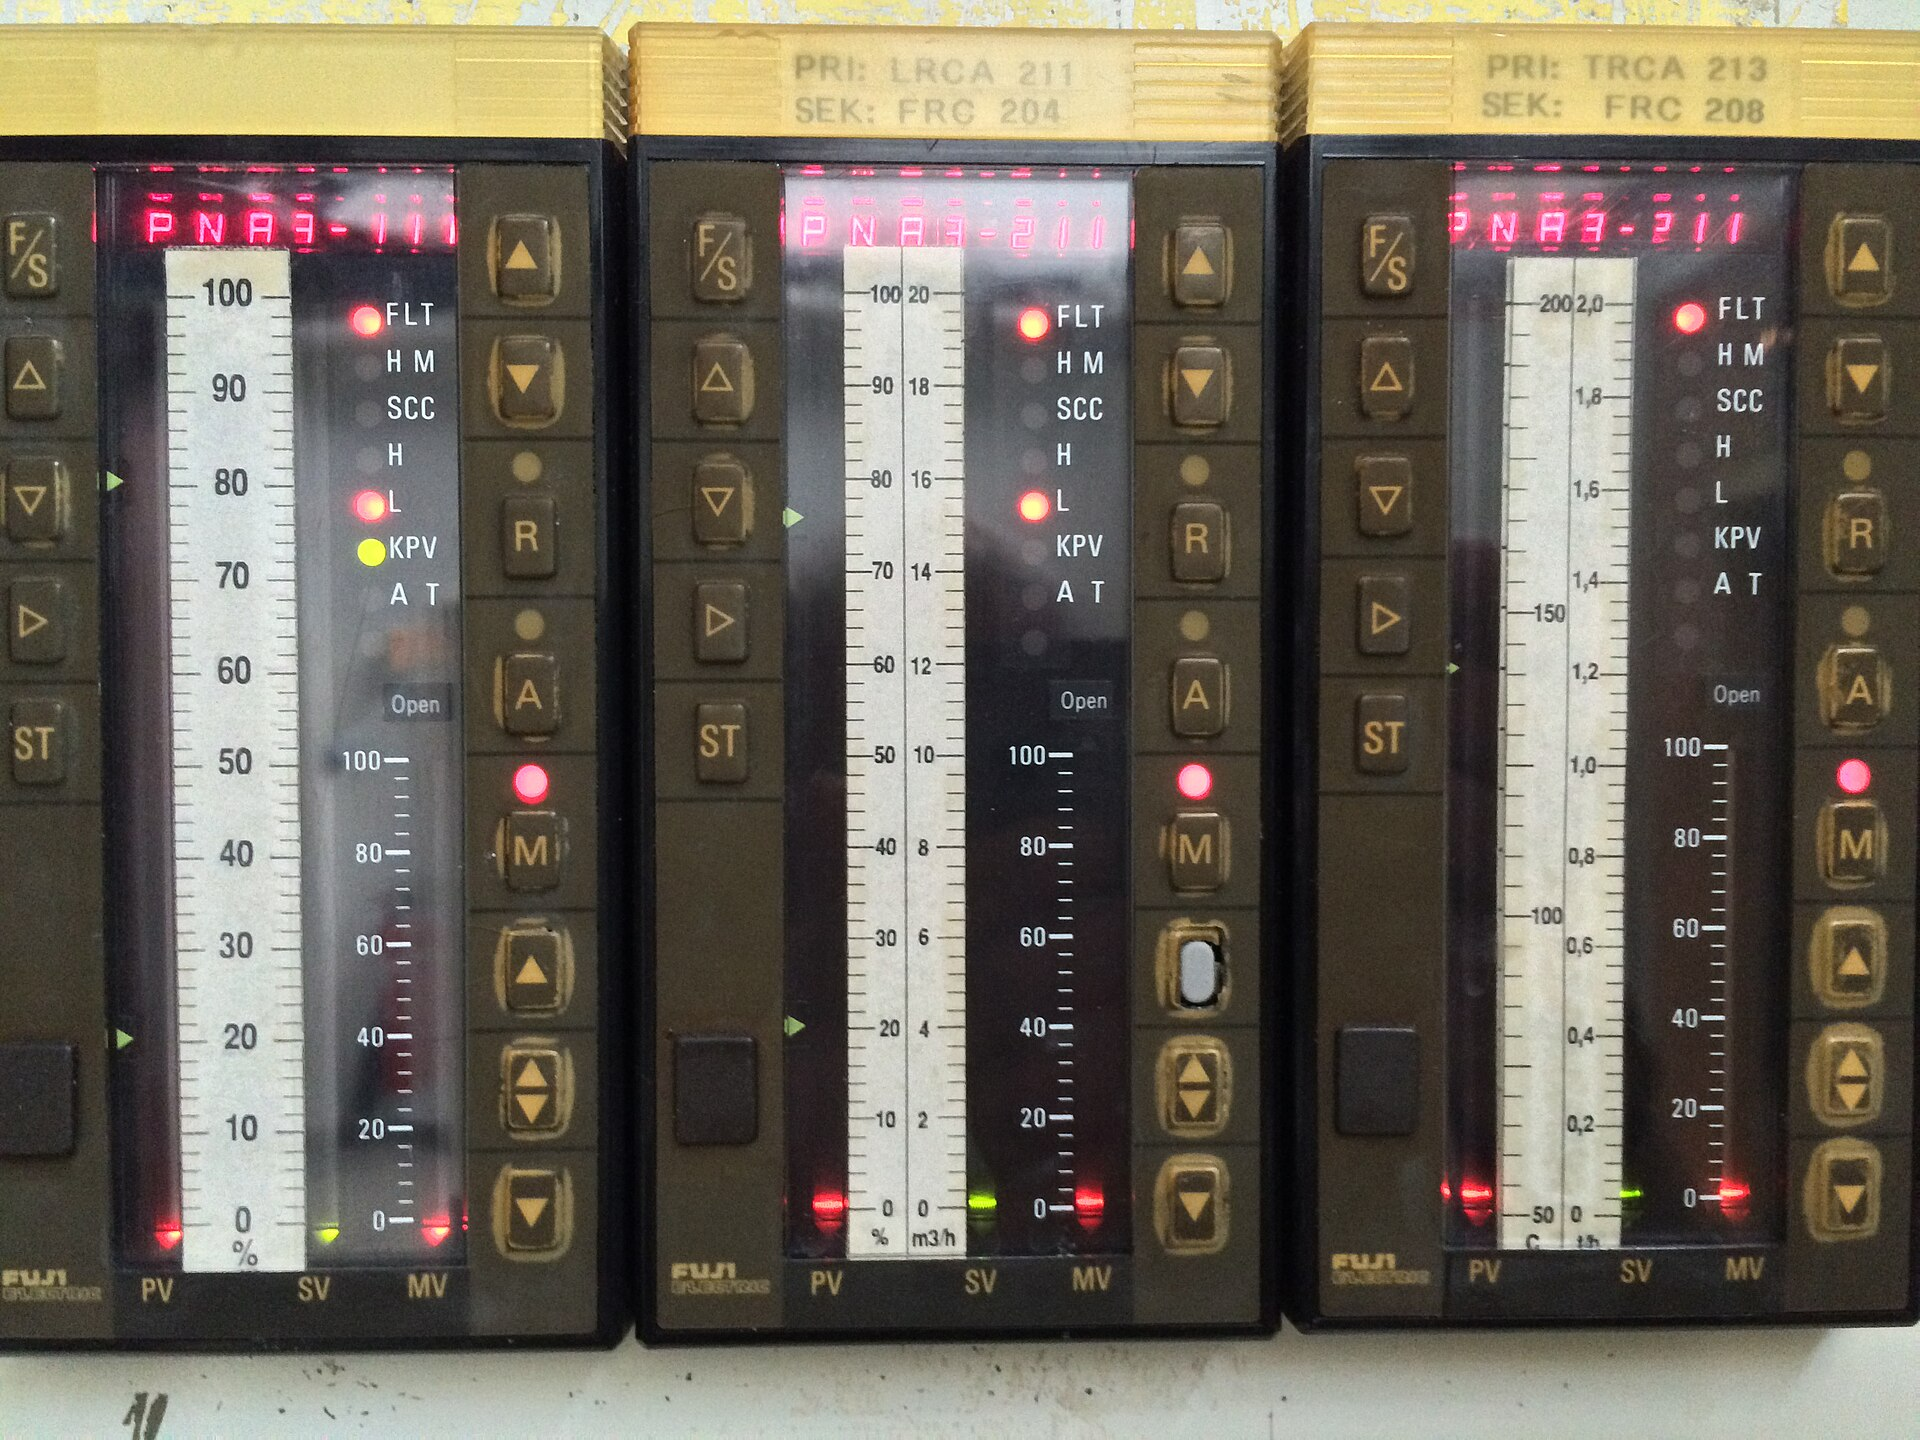
\includegraphics[width=\linewidth]{../../figures/d2_pid_controllers.jpg}\\
\credit{Bitjungle, CC BY-SA 4.0, via Wikimedia Commons}\\[1mm]
\footnotesize\raggedright
Industrial PID controllers usually ask for $K_p$, $T_i$, $T_d$ (ideal form).
\end{columns}
\end{frame}

% ---------------------------------------------------------------------
\begin{frame}{Derivative action: always filter it}
\begin{columns}[T]
\column{.5\textwidth}
\centering
\begin{tikzpicture}
\begin{axis}[mkplot,width=7.0cm,height=5.0cm,xmode=log,xmin=0.01,xmax=1000,ymin=-30,ymax=50,
  xlabel={$\omega T_d$},ylabel={gain of D-part [dB]},legend pos=north west]
  \addplot[mkRed,thick,dashed,domain=-2:3,samples=100] ({10^x},{20*x}); \addlegendentry{ideal $K_pT_ds$}
  \addplot[mkBlue,very thick,domain=-2:3,samples=150] ({10^x},{20*x-10*log10(1+(10^x/10)^2)}); \addlegendentry{filtered, $N=10$}
  \addplot[mkOrange,thick,domain=-2:3,samples=150] ({10^x},{20*x-10*log10(1+(10^x/5)^2)}); \addlegendentry{filtered, $N=5$}
  \node[font=\tiny,anchor=west] at (axis cs:15,26) {limit $20\log N$};
\end{axis}
\end{tikzpicture}
\column{.48\textwidth}
\small
A pure derivative amplifies fast wiggles without limit: sensor noise becomes huge.
\begin{eqbox}
\[
D(s)=\frac{K_pT_d\,s}{1+T_ds/N},\qquad N\approx5\ldots20
\]
\end{eqbox}
\footnotesize
\begin{itemize}
  \item The filter caps the high-frequency D-gain at $K_pN$.
  \item \hl{Derivative on measurement} ($-\dot y$ instead of $\dot e$): no ``kick'' when the target jumps.
  \item Encoder example: 20-bit encoder, 125\,$\mu$s sampling: one count gives a speed jump of 0.048\,rad/s.
\end{itemize}
\end{columns}
\end{frame}

% ---------------------------------------------------------------------
\begin{frame}{Tuning recipe 1: by hand on the robot joint}
\begin{columns}[T]
\column{.5\textwidth}
\begin{defbox}[Step-by-step hand tuning]
\footnotesize
\begin{enumerate}
  \item Start safely: low speed, small steps, $K_i=K_d=0$, limits active.
  \item Raise $K_p$ until the response is fast but starts to ring.
  \item Raise $K_d$ until the ringing is gone ($\approx5$\,\% overshoot).
  \item Add a little $K_i$ to remove the gravity sag; stop when overshoot grows.
  \item Re-check with the heaviest payload and in the worst pose.
\end{enumerate}
\end{defbox}
\footnotesize
Rule of thumb: halve any gain that makes the motor \hl{sing} (audible high-frequency noise).
\column{.47\textwidth}
\centering
\begin{tikzpicture}[font=\scriptsize]
  \draw[-{Latex},thick,mkNavy] (0,0)--(5.2,0) node[below left]{$K_p$};
  \draw[-{Latex},thick,mkNavy] (0,0)--(0,3.6) node[below left,rotate=90,anchor=south east]{$K_d$};
  \fill[mkPale] (1.2,0.9) .. controls (2.5,1.2) and (3.5,1.9) .. (4.4,2.8) -- (4.6,2.0) .. controls (3.5,1.2) and (2.5,0.7) .. (1.3,0.4) -- cycle;
  \node[mkBlue,align=center] at (3.3,1.55) {good};
  \node[mkRed,align=center] at (3.9,.45) {rings};
  \node[mkOrange,align=center] at (1.4,2.8) {sluggish,\\noisy};
  \node[mkGray,align=center] at (.75,.3) {slow};
  \draw[-{Latex},mkOrange,very thick] (.3,.1)--(3.0,.1);
  \draw[-{Latex},mkOrange,very thick] (3.0,.1)--(3.0,1.35);
  \node[mkOrange] at (1.7,.3) {step 2};
  \node[mkOrange,anchor=west] at (3.05,.75) {step 3};
\end{tikzpicture}\\[1mm]
\footnotesize\raggedright
A stiffer joint (higher $K_p$) needs a proportionally larger $K_d$: keep $\zeta$ near 0.7.
\end{columns}
\end{frame}

% ---------------------------------------------------------------------
\begin{frame}{Tuning recipe 2: Ziegler--Nichols (1942)}
\begin{columns}[T]
\column{.46\textwidth}
\small
\textbf{Recipe:} use P only, raise $K_p$ until the loop just keeps oscillating. Note this \term{ultimate gain} $K_u$ and the period $T_u$.
\begin{center}
\footnotesize
\begin{tabular}{@{}lccc@{}}
\toprule
 & $K_p$ & $T_i$ & $T_d$\\
\midrule
P & $0.5K_u$ & -- & --\\
PI & $0.45K_u$ & $T_u/1.2$ & --\\
PID & $0.6K_u$ & $T_u/2$ & $T_u/8$\\
\bottomrule
\end{tabular}
\end{center}
\further{model-based rules (SIMC, lambda tuning) choose a desired closed-loop time constant instead [Skogestad, 2003].}
\column{.52\textwidth}
\begin{defbox}[Worked example]
\footnotesize
Plant $G=1/(s+1)^3$.
\begin{enumerate}
  \item Each pole lags up to $90^\circ$; total $-180^\circ$ when $3\arctan\omega=180^\circ$ $\Rightarrow$ $\omega_u=\sqrt3=1.73$\,rad/s.
  \item There $|G|=1/(1+3)^{3/2}=1/8$ $\Rightarrow$ $K_u=8$.
  \item $T_u=2\pi/1.73=3.63$\,s.
  \item PID: $K_p=4.8$, $T_i=1.81$\,s, $T_d=0.45$\,s.
\end{enumerate}
\end{defbox}
\begin{keybox}[Caution]
\footnotesize
Gives fast but \hl{aggressive} loops. Pushing a real robot to oscillation can be unsafe: use ZN only as a starting point [\AA str\"om \& H\"agglund, 2006].
\end{keybox}
\end{columns}
\end{frame}

% ---------------------------------------------------------------------
\begin{frame}{Saturation and integrator windup}
\begin{columns}[T]
\column{.56\textwidth}
\centering
\begin{tikzpicture}
\begin{groupplot}[group style={group size=1 by 2,vertical sep=3mm,x descriptions at=edge bottom},
  mkplot,width=8.0cm,height=3.7cm,xmin=0,xmax=12]
\nextgroupplot[ylabel={output $y$},ymin=0,ymax=1.3,legend pos=south east,legend columns=3]
  \addplot[mkRed,thick] table[x=t,y=ynone] {data/windup.dat}; \addlegendentry{no anti-windup}
  \addplot[mkOrange,thick,dashed] table[x=t,y=yclamp] {data/windup.dat}; \addlegendentry{clamping}
  \addplot[mkBlue,very thick,dotted] table[x=t,y=ybc] {data/windup.dat}; \addlegendentry{back-calc.}
\nextgroupplot[ylabel={$u$, $v$},xlabel={time [s]},ymin=-2,ymax=4.5]
  \addplot[mkSky,thin] table[x=t,y=vnone] {data/windup.dat};
  \addplot[mkRed,thick] table[x=t,y=unone] {data/windup.dat};
  \addplot[mkOrange,thick,dashed] table[x=t,y=uclamp] {data/windup.dat};
  \addplot[mkBlue,very thick,dotted] table[x=t,y=ubc] {data/windup.dat};
  \addplot[mkGray,dashed,domain=0:12] {1.2};\addplot[mkGray,dashed,domain=0:12] {-1.2};
  \node[font=\tiny,mkSky,anchor=west] at (axis cs:2.5,3.3) {controller wish $v$ (no anti-windup)};
\end{groupplot}
\end{tikzpicture}\\
\footnotesize Plant $1/(s+1)$, PI $K_p=4$, $T_i=0.8$\,s, limit $|u|\le1.2$.
\column{.42\textwidth}
\small
Every real actuator has a \term{saturation}: the drive's current limit, the motor's torque limit.
\footnotesize
\begin{itemize}
  \item Joint blocked by an obstacle, or a long fast move: torque stuck at the limit.
  \item The integrator keeps adding up error although the torque \hl{cannot} grow: it ``winds up''.
  \item When freed, it must first ``unwind'' $\Rightarrow$ big overshoot (18\,\% here) and slow settling.
\end{itemize}
\begin{notebox}
\footnotesize A wound-up joint can \hl{lunge} when the obstacle is removed -- a safety issue.
\end{notebox}
\end{columns}
\end{frame}

% ---------------------------------------------------------------------
\begin{frame}{Anti-windup: two standard cures}
\begin{columns}[T]
\column{.55\textwidth}
\centering
\begin{tikzpicture}[node distance=5mm]
  \node[sum] (s1) {};
  \node[blk,right=8mm of s1] (P) {$K_p$};
  \node[blk,below=4mm of P] (I) {$\dfrac{K_i}{s}$};
  \node[sum,right=8mm of P] (s2) {};
  \node[blko,right=6mm of s2,minimum width=12mm] (sat) {};
  \draw[thick,mkNavy] ($(sat.center)+(-.45,-.22)$)--($(sat.center)+(-.15,-.22)$)--($(sat.center)+(.15,.22)$)--($(sat.center)+(.45,.22)$);
  \draw[sig] ($(s1.west)-(5mm,0)$) node[left,lbl]{$e$}--(s1);
  \draw[sig] (s1)--(P); \fill ($(s1.east)+(3mm,0)$) circle (1pt);
  \draw[sig] ($(s1.east)+(3mm,0)$) |- (I);
  \draw[sig] (P)--(s2); \draw[sig] (I) -| (s2);
  \draw[sig] (s2)--(sat) node[midway,above,lbl]{$v$};
  \draw[sig] (sat)--++(14mm,0) node[right,lbl]{$u$};
  \node[sum,below=8mm of sat] (s3) {};
  \fill ($(sat.east)+(6mm,0)$) circle (1pt);
  \draw[sig,mkOrange] ($(sat.east)+(6mm,0)$) |- (s3) node[pos=.8,above,lbl]{$+$};
  \fill ($(s2.east)+(2mm,0)$) circle (1pt);
  \draw[sig,mkOrange] ($(s2.east)+(2mm,0)$) |- (s3) node[pos=.85,above,lbl]{$-$};
  \node[blko,below=4mm of s3] (Tt) {$1/T_t$};
  \draw[sig,mkOrange] (s3)--(Tt);
  \draw[sig,mkOrange] (Tt) -| (s1.south|-I.south) -- ($(I.west)+(0,-1.5mm)$);
  \node[lbl,text=mkOrange,anchor=north] at ($(Tt.south)+(0,-.5mm)$) {back-calculation path};
\end{tikzpicture}
\column{.43\textwidth}
\small
\begin{defbox}[Clamping]
\footnotesize
Stop integrating while the output is at its limit \emph{and} the error pushes further. Simple; standard in servo drives.
\end{defbox}
\begin{defbox}[Back-calculation]
\footnotesize
Feed the difference $u-v$ (actual minus wished) back into the integrator, scaled by $1/T_t$, so it tracks the limit. Typical $T_t\approx T_i/2$.
\end{defbox}
\footnotesize
\hl{Every} controller with an integrator and a saturating actuator needs one of these.
\further{in cascaded loops, pass the inner loop's limit to the outer integrator.}
\end{columns}
\end{frame}

% ---------------------------------------------------------------------
\begin{frame}{Feedforward: let feedback correct only what is unknown}
\begin{columns}[T]
\column{.5\textwidth}
\centering
\begin{tikzpicture}[node distance=5mm,scale=.85,transform shape]
  \node[blk] (traj) {trajectory\\generator};
  \node[sum,right=8mm of traj] (s1) {};
  \node[blk,right=of s1] (C) {$C(s)$};
  \node[sum,right=of C] (s2) {};
  \node[blk,right=of s2] (G) {$G=\frac{1}{Js^2+Bs}$};
  \node[blko,above=5mm of C] (F) {$\hat J\ddot\theta_r+\hat B\dot\theta_r$};
  \draw[sig] (traj)--(s1) node[midway,above,lbl]{$\theta_r$};
  \draw[sig] (s1)--(C); \draw[sig] (C)--(s2); \draw[sig] (s2)--(G);
  \draw[sig] (G)--++(11mm,0) node[above,lbl]{$\theta$};
  \draw[sig] (traj.north) |- (F) node[pos=.3,left,lbl]{$\dot\theta_r,\ddot\theta_r$};
  \draw[sig] (F) -| (s2) node[pos=.9,left,lbl]{$+$};
  \fill ($(G.east)+(6mm,0)$) circle (1pt);
  \draw[sig] ($(G.east)+(6mm,0)$)--++(0,-9mm) -| (s1) node[pos=.95,left,lbl]{$-$};
\end{tikzpicture}\\[2mm]
\small\raggedright
A driver who \emph{sees} the hill presses the pedal \hl{before} the car slows: that is feedforward.
\begin{eqbox}
\[
T_{\mathrm{FF}}=\hat J\,\ddot\theta_r+\hat B\,\dot\theta_r\;(+\,\hat T_g)
\]
\end{eqbox}
\column{.48\textwidth}
\centering
\begin{tikzpicture}
\begin{axis}[mkplot,width=7.0cm,height=4.8cm,xlabel={time [ms]},ylabel={tracking error [mrad]},
  xmin=0,xmax=600,ymin=-10,ymax=10,legend pos=north east,legend cell align=left]
  \addplot[mkRed,thick] table[x=t,y=e_fb] {data/feedforward.dat}; \addlegendentry{feedback only (8.8\,mrad)}
  \addplot[mkOrange,thick] table[x=t,y=e_ff90] {data/feedforward.dat}; \addlegendentry{FF, $\hat J=0.9J$ (0.86\,mrad)}
  \addplot[mkBlue,very thick,dashed] table[x=t,y=e_ff100] {data/feedforward.dat}; \addlegendentry{FF, $\hat J=J$ ($\approx0$)}
\end{axis}
\end{tikzpicture}\\
\footnotesize
\begin{itemize}
  \item Even with a 10\,\% inertia error: $10\times$ smaller error.
  \item FF sits outside the loop: it does \hl{not} affect stability.
  \item Needs a smooth reference (S-curve profile, W1D5).
\end{itemize}
\end{columns}
\end{frame}

% ---------------------------------------------------------------------
\begin{frame}{Session 2.5 -- Check your understanding}
\begin{columns}[T]
\column{.62\textwidth}
\begin{keybox}[Check your understanding]
\begin{enumerate}
  \item A PD-controlled joint ($K_p=200$\,Nm/rad) holds a 10\,Nm gravity load. How large is the sag? Which term removes it?
  \item Why do we always filter the D-term?
  \item A gripper closes on a part and is blocked for 2\,s with the torque at its limit. What happens inside a PI controller without anti-windup?
\end{enumerate}
\end{keybox}
\column{.35\textwidth}
\centering
\begin{tikzpicture}[scale=.9,font=\scriptsize]
  \fill[mkGray!40] (-.5,-.3) rectangle (.5,0);
  \draw[thick,fill=mkPale,draw=mkBlue] (0,.25) circle (.25);
  \draw[line width=5pt,mkMid] (0,.25)--(2.8,.25);
  \draw[line width=5pt,mkMid,dashed] (0,.25)--(2.75,-.25);
  \fill[mkOrange] (2.8,.25) circle (.2);
  \draw[-{Latex},thick,mkRed] (2.8,.0)--(2.8,-.9) node[below]{$10$\,Nm load};
  \node[mkGray] at (1.4,.7) {target};
  \node[mkGray] at (1.2,-.45) {sag?};
\end{tikzpicture}
\end{columns}
\end{frame}

% ---------------------------------------------------------------------
\begin{frame}{Session 2.5 -- Summary and key terms}
\begin{columns}[T]
\column{.55\textwidth}
\begin{keybox}[Key take-aways]
\footnotesize
\begin{itemize}
  \item P = virtual spring, D = virtual damper, I = learns constant loads (gravity).
  \item Pick $K_p=J\omega_n^2$, $K_d\approx2\zeta\omega_nJ$ as a starting point.
  \item Filter D; apply it to the measurement.
  \item Every saturating integrator needs \hl{anti-windup}.
  \item Feedforward (inertia, friction, gravity) improves tracking without changing stability.
\end{itemize}
\end{keybox}
\column{.42\textwidth}
\begin{defbox}[Key terms]
\footnotesize
\term{PID}: proportional--integral--derivative.\\
\term{Integral time} $T_i$, \term{derivative time} $T_d$.\\
\term{Saturation}: actuator at its limit.\\
\term{Windup}: integrator grows while saturated.\\
\term{Feedforward}: act on the known command before an error appears.
\end{defbox}
\end{columns}
\end{frame}

% =====================================================================
\section{2.6 Stability and Performance}
% =====================================================================

\begin{frame}{What does ``stable'' mean?}
\begin{columns}[T]
\column{.5\textwidth}
\centering
\begin{tikzpicture}[font=\scriptsize]
  \draw[very thick,mkBlue] (-1,0.8) parabola bend (0,0) (1,0.8);
  \fill[mkOrange] (0,0.15) circle (.15);
  \node[align=center] at (0,-.5) {\textbf{stable}\\returns};
  \begin{scope}[xshift=2.6cm]
    \draw[very thick,mkBlue] (-1,0) parabola bend (0,0.8) (1,0);
    \fill[mkOrange] (0,0.95) circle (.15);
    \node[align=center] at (0,-.5) {\textbf{unstable}\\runs away};
  \end{scope}
  \begin{scope}[xshift=5.2cm]
    \draw[very thick,mkBlue] (-1,0.1)--(1,0.1);
    \fill[mkOrange] (0,0.25) circle (.15);
    \node[align=center] at (0,-.5) {\textbf{marginal}\\stays where pushed};
  \end{scope}
\end{tikzpicture}\\[3mm]
\footnotesize\raggedright
Shower analogy: the hot water arrives late (delay). If you over-react to what you feel now, the temperature swings ever more -- \hl{feedback can create instability}.
\column{.48\textwidth}
\small
Closed-loop poles are the roots of the \term{characteristic equation} $1+L(s)=0$.
\begin{eqbox}
\[
\text{stable}\iff\text{all poles: }\operatorname{Re}(p)<0
\]
\end{eqbox}
\footnotesize
\textbf{Example} $L(s)=\dfrac{K}{s(s+2)(s+5)}$:
\begin{enumerate}
  \item $1+L=0$ $\Rightarrow$ $s^3+7s^2+10s+K=0$
  \item $K=20$: poles $-5.88$ and $-0.56\pm j1.76$ $\Rightarrow$ stable
  \item $K=100$: two poles in the right half-plane $\Rightarrow$ unstable
\end{enumerate}
Too much gain destabilises -- we will see why on the next slides.
\end{columns}
\end{frame}

% ---------------------------------------------------------------------
\begin{frame}{Time-domain specifications}
\begin{columns}[T]
\column{.56\textwidth}
\centering
\begin{tikzpicture}
\begin{axis}[mkplot,width=8.2cm,height=5.6cm,xlabel={$\omega_nt$},ylabel={$y(t)$},xmin=0,xmax=14,ymin=0,ymax=1.4]
  \fill[mkPale] (axis cs:0,0.98) rectangle (axis cs:14,1.02);
  \addplot[mkBlue,very thick,domain=0:14,samples=250] {1-exp(-0.4*x)/sqrt(1-0.16)*sin(deg(sqrt(1-0.16)*x)+acos(0.4))};
  \addplot[mkGray,dashed,domain=0:14] {1};
  \draw[mkOrange,dashed] (axis cs:0.48,0)--(axis cs:0.48,0.1); \draw[mkOrange,dashed] (axis cs:1.94,0)--(axis cs:1.94,0.9);
  \draw[mkOrange,thick,<->] (axis cs:0.48,0.05)--(axis cs:1.94,0.05) node[midway,above,font=\tiny]{$t_r$};
  \draw[mkMid,dashed] (axis cs:3.43,0)--(axis cs:3.43,1.254);
  \node[font=\tiny,anchor=north west] at (axis cs:3.43,0.2) {$t_p$};
  \draw[mkOrange,thick,<->] (axis cs:4.2,1)--(axis cs:4.2,1.254) node[midway,right,font=\tiny]{$M_p=25\,\%$};
  \draw[mkMid,dashed] (axis cs:8.41,0)--(axis cs:8.41,0.98);
  \node[font=\tiny,anchor=north west] at (axis cs:8.41,0.45) {$t_s$ (2\,\%)};
  \node[font=\tiny,anchor=south east] at (axis cs:14,0.62) {$\zeta=0.4$};
\end{axis}
\end{tikzpicture}
\column{.42\textwidth}
\footnotesize
\begin{tabular}{@{}p{1.9cm}p{3.0cm}@{}}
\toprule
Measure & Meaning\\
\midrule
Rise time $t_r$ & 10\,\% $\rightarrow$ 90\,\%\\
Overshoot $M_p$ & how far past the target\\
Settling time $t_s$ & stays within $\pm2\,\%$\\
Steady-state error & error left at the end\\
\bottomrule
\end{tabular}\\[3pt]
For a 2nd-order closed loop, \hl{$\zeta$ alone fixes the overshoot}:
\begin{eqbox}
\[
M_p=e^{-\pi\zeta/\sqrt{1-\zeta^2}},\qquad t_s\approx\frac{4}{\zeta\omega_n}
\]
\end{eqbox}
\begin{tabular}{@{}lccccc@{}}
\toprule
$\zeta$ & 0.3 & 0.4 & 0.5 & 0.6 & 0.7\\
\midrule
$M_p$ [\%] & 37 & 25 & 16 & 9.5 & 4.6\\
PM [deg] & 33 & 43 & 52 & 59 & 65\\
\bottomrule
\end{tabular}\\[2pt]
Robot pick-and-place: usually $M_p<5\,\%$ (do not hit the table!).
\end{columns}
\end{frame}

% ---------------------------------------------------------------------
\begin{frame}{From specifications to pole positions}
\begin{columns}[T]
\column{.5\textwidth}
\centering
\begin{tikzpicture}[scale=.68,font=\scriptsize]
  \clip (-4.6,-3.1) rectangle (1.6,3.3);
  \fill[mkRed!15] (0,-3) rectangle (1.6,3.1);
  \fill[mkPale] (-1.2,-1.224) -- (-1.2,1.224) -- (-4.6,4.69) -- (-4.6,-4.69) -- cycle;
  \draw[-{Latex},mkGray] (-4.6,0)--(1.5,0) node[above left]{Re};
  \draw[-{Latex},mkGray] (0,-3.0)--(0,3.1) node[below left]{Im};
  \draw[mkOrange,very thick] (0,0)--(-3.1,3.16); \draw[mkOrange,very thick] (0,0)--(-3.1,-3.16);
  \draw[mkBlue,very thick,dashed] (-1.2,-3)--(-1.2,3);
  \node[mkOrange,anchor=east] at (-2.0,2.7) {$\zeta=0.7$};
  \node[mkBlue,anchor=west] at (-1.15,-2.6) {$-4/t_s$};
  \node[mkNavy,font=\scriptsize\bfseries] at (-3.2,0.35) {good poles};
  \draw[mkRed,very thick] (0.8,1.2)++(-.12,-.12)--++(.24,.24) (0.8,1.2)++(-.12,.12)--++(.24,-.24);
  \node[mkRed] at (0.8,1.75) {unstable};
  \draw[mkGray,very thick] (-.5,2.2)++(-.12,-.12)--++(.24,.24) (-.5,2.2)++(-.12,.12)--++(.24,-.24);
  \node[mkGray,anchor=west] at (-.3,2.75) {ringing};
  \draw[mkBlue,very thick] (-2.0,1.4)++(-.12,-.12)--++(.24,.24) (-2.0,1.4)++(-.12,.12)--++(.24,-.24);
  \draw[mkBlue,very thick] (-2.0,-1.4)++(-.12,-.12)--++(.24,.24) (-2.0,-1.4)++(-.12,.12)--++(.24,-.24);
\end{tikzpicture}
\column{.48\textwidth}
\small
Each spec draws a line in the $s$-plane; good poles sit in the \hl{shaded wedge}.
\footnotesize
\begin{itemize}
  \item Overshoot $\Rightarrow$ $\zeta\ge\zeta_{\min}$: inside the \textcolor{mkOrange}{angle lines}.
  \item Settling $\Rightarrow$ real part $\le-4/t_s$: left of the \textcolor{mkBlue}{dashed line}.
\end{itemize}
\begin{defbox}[Worked example]
\footnotesize
Joint must settle in $t_s=0.4$\,s with $<5$\,\% overshoot.
\begin{enumerate}
  \item $\zeta\ge0.7$; $\zeta\omega_n\ge4/0.4=10$\,s$^{-1}$.
  \item $\omega_n\ge10/0.7=14.3$\,rad/s.
  \item $K_p=J\omega_n^2=0.5\cdot204=102$\,Nm/rad.
\end{enumerate}
\end{defbox}
\end{columns}
\end{frame}

% ---------------------------------------------------------------------
\begin{frame}{Steady-state error and system type}
\begin{columns}[T]
\column{.48\textwidth}
\small
Final value theorem (only for a \hl{stable} loop):
\begin{eqbox}
\[
e_\infty=\lim_{t\rightarrow\infty}e(t)=\lim_{s\rightarrow0}s\,E(s),\quad E=\frac{R}{1+L}
\]
\end{eqbox}
\footnotesize
\term{System type} = number of integrators ($1/s$) in $L(s)$.
\begin{center}
\begin{tabular}{@{}lccc@{}}
\toprule
Type & step & ramp & example\\
\midrule
0 & $\frac{1}{1+L(0)}$ & $\infty$ & cruise control, P only\\[3pt]
1 & 0 & $\frac{1}{K_v}$ & PI, or position loop\\[3pt]
2 & 0 & 0 & position loop + I\\
\bottomrule
\end{tabular}
\end{center}
$K_v=\lim_{s\rightarrow0}sL(s)$ [s$^{-1}$], the velocity constant.
\column{.5\textwidth}
\begin{defbox}[Worked example: gantry axis following error]
\footnotesize
\begin{enumerate}
  \item Position P gain $K_{pp}=126$\,s$^{-1}$ around a fast speed loop: $L\approx K_{pp}/s$ $\Rightarrow$ type 1, $K_v=126$\,s$^{-1}$.
  \item Axis moves at 0.2\,m/s, 10\,mm ball-screw pitch $\Rightarrow$ motor speed $\dot\theta=126$\,rad/s (a ramp in $\theta$).
  \item $e_\infty=\dot\theta/K_v=126/126=1$\,rad.
  \item $1$\,rad $\times10\,\mathrm{mm}/2\pi=1.6$\,mm lag behind the command.
\end{enumerate}
\end{defbox}
\footnotesize
Cure: velocity feedforward (session 2.5) removes this lag. Gravity on a P-only joint is a type-0 \hl{step disturbance}.
\end{columns}
\end{frame}

% ---------------------------------------------------------------------
\begin{frame}{Root locus: how closed-loop poles move with gain}
\begin{columns}[T]
\column{.52\textwidth}
\centering
\begin{tikzpicture}
\begin{axis}[mkplot,width=7.4cm,height=6.0cm,xlabel={Re},ylabel={Im},xmin=-9,xmax=3,ymin=-5,ymax=5,
  axis lines=middle,xlabel style={anchor=north east,at={(rel axis cs:1,0.5)}},
  ylabel style={anchor=south,at={(rel axis cs:0.75,1)}}]
  \addplot[mkBlue,very thick] table[x=r1,y=i1] {data/rlocus.dat};
  \addplot[mkBlue,very thick] table[x=r2,y=i2] {data/rlocus.dat};
  \addplot[mkBlue,very thick] table[x=r3,y=i3] {data/rlocus.dat};
  \addplot[only marks,mark=x,mark size=3pt,mkNavy,very thick] coordinates {(0,0)(-2,0)(-5,0)};
  \addplot[only marks,mark=*,mark size=1.8pt,mkOrange] coordinates {(-0.561,1.757)(-0.561,-1.757)(-5.878,0)};
  \addplot[only marks,mark=square*,mark size=1.6pt,mkRed] coordinates {(0,3.162)(0,-3.162)};
  \node[font=\tiny,mkOrange,anchor=east] at (axis cs:-1.2,1.6) {$K=20$};
  \node[font=\tiny,mkRed,anchor=west] at (axis cs:0.15,3.162) {$K=70$};
  \node[font=\tiny,mkNavy,anchor=north] at (axis cs:-2,-0.2) {$K=0$};
\end{axis}
\end{tikzpicture}
\column{.46\textwidth}
\small
Same loop $L=\dfrac{K}{s(s+2)(s+5)}$; the curves show where the 3 closed-loop poles go as $K$ grows from 0.
\footnotesize
\begin{itemize}
  \item $K=0$: poles start at the open-loop poles $0,-2,-5$ ($\times$).
  \item Small $K$: two poles meet and split into a complex pair $\Rightarrow$ oscillation starts.
  \item $K=20$: $-0.56\pm j1.76$ ($\zeta=0.30$, $\approx$\,37\,\% overshoot).
  \item $K=70$: poles reach the $j\omega$-axis at $\pm j3.16$ $\Rightarrow$ \hl{stability limit}.
  \item $K>70$: unstable.
\end{itemize}
\further{the Routh--Hurwitz table gives the same limit $0<K<70$ from the coefficients alone; the Nyquist plot of $L(j\omega)$ must not encircle $-1$.}
\end{columns}
\end{frame}

% ---------------------------------------------------------------------
\begin{frame}{Gain and phase margins: how far from the edge?}
\begin{columns}[T]
\column{.55\textwidth}
\centering
\begin{tikzpicture}
\begin{groupplot}[group style={group size=1 by 2,vertical sep=4mm,x descriptions at=edge bottom},
  mkplot,width=8.0cm,height=3.9cm,xmode=log,xmin=0.1,xmax=100]
\nextgroupplot[ylabel={$|L|$ [dB]},ymin=-60,ymax=50]
  \addplot[mkBlue,very thick] table[x=w,y=mag] {data/loop_bode.dat};
  \addplot[mkGray,dashed,domain=0.1:100] {0};
  \draw[mkOrange,very thick,<->] (axis cs:3.17,0)--(axis cs:3.17,-10.9) node[midway,right,font=\tiny]{GM $=10.9$\,dB};
  \fill[mkNavy] (axis cs:1.515,0) circle (1.5pt);
  \node[font=\tiny,anchor=south west] at (axis cs:1.55,0.5) {$\omega_c=1.52$};
\nextgroupplot[ylabel={$\angle L$ [deg]},xlabel={$\omega$ [rad/s]},ymin=-270,ymax=-80,ytick={-270,-225,-180,-135,-90}]
  \addplot[mkBlue,very thick] table[x=w,y=ph] {data/loop_bode.dat};
  \addplot[mkGray,dashed,domain=0.1:100] {-180};
  \draw[mkOrange,very thick,<->] (axis cs:1.515,-180)--(axis cs:1.515,-144) node[midway,left,font=\tiny]{PM $=36^\circ$};
  \fill[mkNavy] (axis cs:3.17,-180) circle (1.5pt);
  \node[font=\tiny,anchor=north west] at (axis cs:3.2,-182) {$\omega_{180}=3.16$};
\end{groupplot}
\end{tikzpicture}
\column{.43\textwidth}
\small
The loop oscillates if a signal comes back around the loop with gain 1 and $-180^\circ$. Margins = \hl{safety distance} from that point.
\footnotesize
\begin{enumerate}
  \item Find the \term{crossover} $\omega_c$ where $|L|=0$\,dB (1.52\,rad/s).
  \item Read the phase there: $-144^\circ$ $\Rightarrow$ \term{phase margin} PM $=180^\circ-144^\circ=36^\circ$.
  \item Find where the phase is $-180^\circ$ (3.16\,rad/s); $|L|=-10.9$\,dB there $\Rightarrow$ \term{gain margin} GM $=10.9$\,dB ($\times3.5$).
\end{enumerate}
\begin{itemize}
  \item Same loop as the root locus with $K=20$: GM $\times3.5$ $\Rightarrow$ $K=70$ is the limit. \hl{Consistent!}
  \item Targets: PM $45$--$60^\circ$, GM $\ge6$\,dB.
\end{itemize}
\end{columns}
\end{frame}

% ---------------------------------------------------------------------
\begin{frame}{Worked example: margins of a joint position loop}
\begin{columns}[T]
\column{.53\textwidth}
\centering
\begin{tikzpicture}
\begin{groupplot}[group style={group size=1 by 2,vertical sep=4mm,x descriptions at=edge bottom},
  mkplot,width=7.8cm,height=3.8cm,xmode=log,xmin=5,xmax=1000]
\nextgroupplot[ylabel={$|L|$ [dB]},ymin=-40,ymax=30]
  \addplot[mkBlue,very thick,domain=0.7:3,samples=120] ({10^x},{40-20*x-10*log10(1+(0.01*10^x)^2)});
  \addplot[mkGray,dashed,domain=5:1000] {0};
  \fill[mkNavy] (axis cs:78.6,0) circle (1.6pt);
  \node[font=\tiny,anchor=south west] at (axis cs:80,1) {$\omega_c=78.6$\,rad/s};
\nextgroupplot[ylabel={$\angle L$ [deg]},xlabel={$\omega$ [rad/s]},ymin=-240,ymax=-80,ytick={-225,-180,-135,-90},
  legend pos=south west,legend cell align=left]
  \addplot[mkBlue,very thick,domain=0.7:3,samples=120] ({10^x},{-90-atan(0.01*10^x)}); \addlegendentry{no delay}
  \addplot[mkOrange,thick,dashed,domain=0.7:3,samples=120] ({10^x},{-90-atan(0.01*10^x)-0.002*10^x*57.3}); \addlegendentry{2\,ms delay}
  \addplot[mkRed,thick,dotted,domain=0.7:3,samples=120] ({10^x},{-90-atan(0.01*10^x)-0.006*10^x*57.3}); \addlegendentry{6\,ms delay}
  \addplot[mkGray,dashed,domain=5:1000] {-180};
  \draw[mkNavy,very thick,<->] (axis cs:78.6,-180)--(axis cs:78.6,-128.2);
  \node[font=\tiny,anchor=west] at (axis cs:85,-150) {PM $52^\circ$};
\end{groupplot}
\end{tikzpicture}
\column{.45\textwidth}
\small
Joint position loop (speed loop inside, lag $\tau=10$\,ms):
\begin{eqbox}
\[
L(s)=\frac{100}{s\,(0.01s+1)}
\]
\end{eqbox}
\footnotesize
\begin{enumerate}
  \item Crossover: $|L|=1$ $\Rightarrow$ $\omega_c\approx78.6$\,rad/s (12.5\,Hz).
  \item Phase: $-90^\circ-\arctan(0.786)=-128.2^\circ$ $\Rightarrow$ PM $=51.8^\circ$.
  \item Phase never reaches $-180^\circ$ $\Rightarrow$ GM is infinite.
  \item A delay $T_d$ removes $\omega_cT_d$ rad: 2\,ms $\Rightarrow$ $-9^\circ$ (PM $43^\circ$); 6\,ms $\Rightarrow$ $-27^\circ$ (PM $25^\circ$).
\end{enumerate}
\end{columns}
\end{frame}

% ---------------------------------------------------------------------
\begin{frame}{Time delay: the shower problem in a robot}
\begin{columns}[T]
\column{.55\textwidth}
\centering
\begin{tikzpicture}
\begin{axis}[mkplot,width=8.0cm,height=5.2cm,xlabel={time [ms]},ylabel={joint angle (normalised)},xmin=0,xmax=150,ymin=0,ymax=1.65,
  legend pos=north east,legend cell align=left]
  \addplot[mkBlue,very thick] table[x=t,y=d0] {data/delay_step.dat}; \addlegendentry{no delay: 16\,\% overshoot}
  \addplot[mkOrange,thick,dashed] table[x=t,y=d2] {data/delay_step.dat}; \addlegendentry{2\,ms: 26\,\%}
  \addplot[mkRed,thick] table[x=t,y=d6] {data/delay_step.dat}; \addlegendentry{6\,ms: 53\,\%}
  \addplot[mkGray,dashed,domain=0:150] {1};
\end{axis}
\end{tikzpicture}\\
\footnotesize Same loop as previous slide, closed with unity feedback; simulated.
\column{.43\textwidth}
\small
Delays come from sampling, computation, filters and \hl{networks} (EtherCAT, CAN: W2D5).
\begin{eqbox}
\[
\Delta\varphi=-\omega_c\,T_d\ \text{[rad]}
\]
\end{eqbox}
\footnotesize
\begin{itemize}
  \item A delay changes \hl{phase only}, not gain: it cannot be seen in $|L|$.
  \item Limit here: $0.904\,\mathrm{rad}/78.6\,\mathrm{rad/s}=11.5$\,ms of delay makes the joint oscillate.
  \item The faster the loop (higher $\omega_c$), the less delay it tolerates.
\end{itemize}
\end{columns}
\end{frame}

% ---------------------------------------------------------------------
\begin{frame}{Sensitivity, robustness and loop shaping}
\begin{columns}[T]
\column{.5\textwidth}
\centering
\begin{tikzpicture}
\begin{axis}[mkplot,width=7.0cm,height=4.2cm,xmode=log,xmin=0.01,xmax=100,ymin=-40,ymax=15,
  xlabel={$\omega$ [rad/s]},ylabel={magnitude [dB]},legend pos=south west]
  \addplot[mkOrange,very thick] table[x=w,y=S] {data/loop_bode.dat}; \addlegendentry{$|S|$}
  \addplot[mkBlue,very thick] table[x=w,y=T] {data/loop_bode.dat}; \addlegendentry{$|T|$}
  \addplot[mkGray,dashed,domain=0.01:100] {0};
  \node[font=\tiny,mkOrange,anchor=south west] at (axis cs:2.2,6.6) {$M_s=2.12$ (6.5\,dB)};
\end{axis}
\end{tikzpicture}
\begin{tikzpicture}
\begin{axis}[mkplot,width=7.0cm,height=3.5cm,xmin=0,xmax=12,ymin=0,ymax=1.9,xlabel={time [s]},ylabel={$y$},
  legend pos=north east,legend columns=3]
  \addplot[mkSky,thick] table[x=t,y=k10] {data/loop_step.dat}; \addlegendentry{$K=10$}
  \addplot[mkBlue,very thick] table[x=t,y=k20] {data/loop_step.dat}; \addlegendentry{$20$}
  \addplot[mkRed,thick] table[x=t,y=k50] {data/loop_step.dat}; \addlegendentry{$50$}
\end{axis}
\end{tikzpicture}
\column{.48\textwidth}
\small
$|S(j\omega)|$ = how much of a disturbance at frequency $\omega$ survives the loop.
\begin{eqbox}
\[
M_s=\max_\omega|S(j\omega)|\quad(\text{aim: }1.2\ldots2)
\]
\end{eqbox}
\footnotesize
\begin{itemize}
  \item Low frequency: $|S|\ll1$ $\Rightarrow$ disturbances removed.
  \item Near crossover: $|S|>1$ $\Rightarrow$ feedback \hl{amplifies} disturbances.
  \item $K=20$: $M_s=2.1$, PM $36^\circ$ $\Rightarrow$ ringing; $K=10$ is calmer.
  \item \term{Loop shaping}: make $|L|$ big at low frequency (tracking), small at high frequency (noise, resonances).
\end{itemize}
\further{waterbed effect: pushing $|S|$ down at some frequencies pushes it up elsewhere.}
\end{columns}
\end{frame}

% ---------------------------------------------------------------------
\begin{frame}{Bandwidth: how fast can the joint follow?}
\begin{columns}[T]
\column{.53\textwidth}
\centering
\begin{tikzpicture}
\begin{axis}[mkplot,width=7.8cm,height=5.0cm,xmode=log,xmin=0.1,xmax=10,ymin=-25,ymax=12,
  xlabel={$\omega/\omega_n$},ylabel={closed loop $|T|$ [dB]},legend pos=south west,legend cell align=left]
  \addplot[mkRed,thick,domain=-1:1,samples=200] ({10^x},{-10*log10((1-10^(2*x))^2+(2*0.2*10^x)^2)}); \addlegendentry{$\zeta=0.2$}
  \addplot[mkBlue,very thick,domain=-1:1,samples=200] ({10^x},{-10*log10((1-10^(2*x))^2+(2*0.7*10^x)^2)}); \addlegendentry{$\zeta=0.7$}
  \addplot[mkSky,thick,dashed,domain=-1:1,samples=200] ({10^x},{-10*log10((1-10^(2*x))^2+(2*1*10^x)^2)}); \addlegendentry{$\zeta=1$}
  \addplot[mkOrange,thick,dashed,domain=0.1:10] {-3};
  \node[font=\tiny,mkOrange,anchor=south west] at (axis cs:0.11,-2.8) {$-3$\,dB line};
  \draw[mkNavy,dashed] (axis cs:1,-25)--(axis cs:1,-3);
\end{axis}
\end{tikzpicture}
\column{.45\textwidth}
\small
\term{Bandwidth} $\omega_{bw}$: highest frequency the closed loop still follows, $|T|\ge-3$\,dB.
\begin{eqbox}
\[
t_r\approx\frac{2.2}{\omega_{bw}}=\frac{0.35}{f_{bw}}
\]
\end{eqbox}
\footnotesize
\begin{itemize}
  \item Rule of thumb: $\omega_{bw}\approx(1\ldots1.6)\,\omega_c$.
  \item Our joint loop: $\omega_c=78.6$\,rad/s, $\omega_{bw}\approx127$\,rad/s (20\,Hz) $\Rightarrow$ $t_r\approx17$\,ms.
  \item Higher bandwidth = faster, but limited by \hl{resonances} ($\omega_{bw}<\omega_r/3$), delay and noise.
\end{itemize}
\end{columns}
\end{frame}

% ---------------------------------------------------------------------
\begin{frame}{Session 2.6 -- Check your understanding}
\begin{columns}[T]
\column{.62\textwidth}
\begin{keybox}[Check your understanding]
\begin{enumerate}
  \item Closed-loop poles at $-1\pm j3$. Stable? Small or large overshoot?
  \item A loop has a phase margin of only $10^\circ$. What would you see in its step response?
  \item A type-1 position loop has $K_v=100$\,s$^{-1}$ and moves at 50\,rad/s. What is the following error?
  \item Crossover is 100\,rad/s, PM $=40^\circ$. How much delay brings it to the edge?
\end{enumerate}
\end{keybox}
\column{.35\textwidth}
\centering
\begin{tikzpicture}[scale=.75]
  \fill[mkPale] (-2.5,-3.4) rectangle (0,3.4);
  \draw[-{Latex},mkGray] (-2.5,0)--(1,0) node[right]{\scriptsize Re};
  \draw[-{Latex},mkGray] (0,-3.4)--(0,3.6) node[above]{\scriptsize Im};
  \foreach \p in {(-1,3),(-1,-3)}{\draw[mkOrange,very thick] \p++(-.12,-.12)--++(.24,.24) \p++(-.12,.12)--++(.24,-.24);}
  \node[font=\scriptsize,left] at (-1.1,3) {$-1+j3$};
  \node[font=\scriptsize,left] at (-1.1,-3) {$-1-j3$};
\end{tikzpicture}
\end{columns}
\end{frame}

% ---------------------------------------------------------------------
\begin{frame}{Session 2.6 -- Summary, design targets and key terms}
\begin{columns}[T]
\column{.36\textwidth}
\begin{keybox}[Key take-aways]
\footnotesize
\begin{itemize}
  \item Stable $\iff$ closed-loop poles in the left half-plane.
  \item $\zeta$ sets overshoot; PM $\approx100\zeta$.
  \item System type sets the steady-state error.
  \item Delay eats phase: $\omega_cT_d$.
  \item Bandwidth sets speed: $t_r\approx0.35/f_{bw}$.
\end{itemize}
\end{keybox}
\column{.3\textwidth}
\footnotesize
\textbf{Typical design targets}\\[2pt]
\begin{tabular}{@{}lc@{}}
\toprule
Quantity & Target\\
\midrule
Phase margin & 45--60$^\circ$\\
Gain margin & $\ge$\,6\,dB\\
$M_s$ & 1.2--2.0\\
Overshoot (position) & 0--5\,\%\\
$\omega_{bw}$ vs.\ resonance & $<\omega_r/3$\\
\bottomrule
\end{tabular}
\column{.31\textwidth}
\begin{defbox}[Key terms]
\footnotesize
\term{Characteristic eq.} $1+L=0$.\\
\term{Crossover} $\omega_c$: $|L|=1$.\\
\term{Phase margin}: extra lag tolerated.\\
\term{Gain margin}: extra gain tolerated.\\
\term{System type}: integrators in $L$.\\
\term{Bandwidth}: $-3$\,dB of $T$.
\end{defbox}
\end{columns}
\end{frame}

% =====================================================================
\section{Wrap-up}
% =====================================================================
\begin{frame}{Day summary}
\begin{columns}[T]
\column{.5\textwidth}
\begin{defbox}[The control design chain]
\footnotesize
model $G(s)$ or $(A,B,C,D)$ $\rightarrow$ block diagram with $C(s)$ $\rightarrow$ Bode plot of $L=CG$ $\rightarrow$ pick PID gains $\rightarrow$ check poles, PM, GM, bandwidth $\rightarrow$ add anti-windup and feedforward.
\end{defbox}
\begin{keybox}[Numbers to remember]
\footnotesize
$-20$\,dB/dec per pole \textbullet\ $-3$\,dB at the corner \textbullet\ $\zeta=0.7$: 5\,\% overshoot \textbullet\ PM 45--60$^\circ$ \textbullet\ GM $\ge$\,6\,dB \textbullet\ $t_r\approx0.35/f_{bw}$
\end{keybox}
\column{.47\textwidth}
\centering
\begin{tikzpicture}[node distance=4mm,font=\scriptsize]
  \node[blk,minimum width=26mm] (a) {2.3 block diagrams,\\state space};
  \node[blk,below=of a,minimum width=26mm] (b) {2.4 Bode plots};
  \node[blko,below=of b,minimum width=26mm] (c) {2.5 PID, windup,\\feedforward};
  \node[blk,below=of c,minimum width=26mm] (d) {2.6 stability,\\margins, bandwidth};
  \draw[sig] (a)--(b); \draw[sig] (b)--(c); \draw[sig] (c)--(d);
  \draw[sig,mkOrange,dashed] (d.east) -- ++(6mm,0) |- (c.east) node[pos=.25,right,text=mkOrange,align=left]{re-tune\\if margins\\too small};
\end{tikzpicture}
\end{columns}
\end{frame}

% ---------------------------------------------------------------------
\begin{frame}{Preview of W1D4: control (cont.) and servo systems I}
\begin{columns}[T]
\column{.55\textwidth}
\small
\begin{itemize}
  \item \textbf{2.7} Filters and compensation: low-pass, notch (for today's resonance), lead/lag.
  \item \textbf{2.8} Digital control: sampling, zero-order hold, discrete PID, delay.
  \item \textbf{2.9} Control of robot manipulators: independent joints, gravity compensation, computed torque.
  \item \textbf{3.1} Servo architecture: torque / velocity / position modes.
  \item \textbf{3.2} Power electronics for drives: DC bus, inverter, PWM.
\end{itemize}
\column{.42\textwidth}
\centering
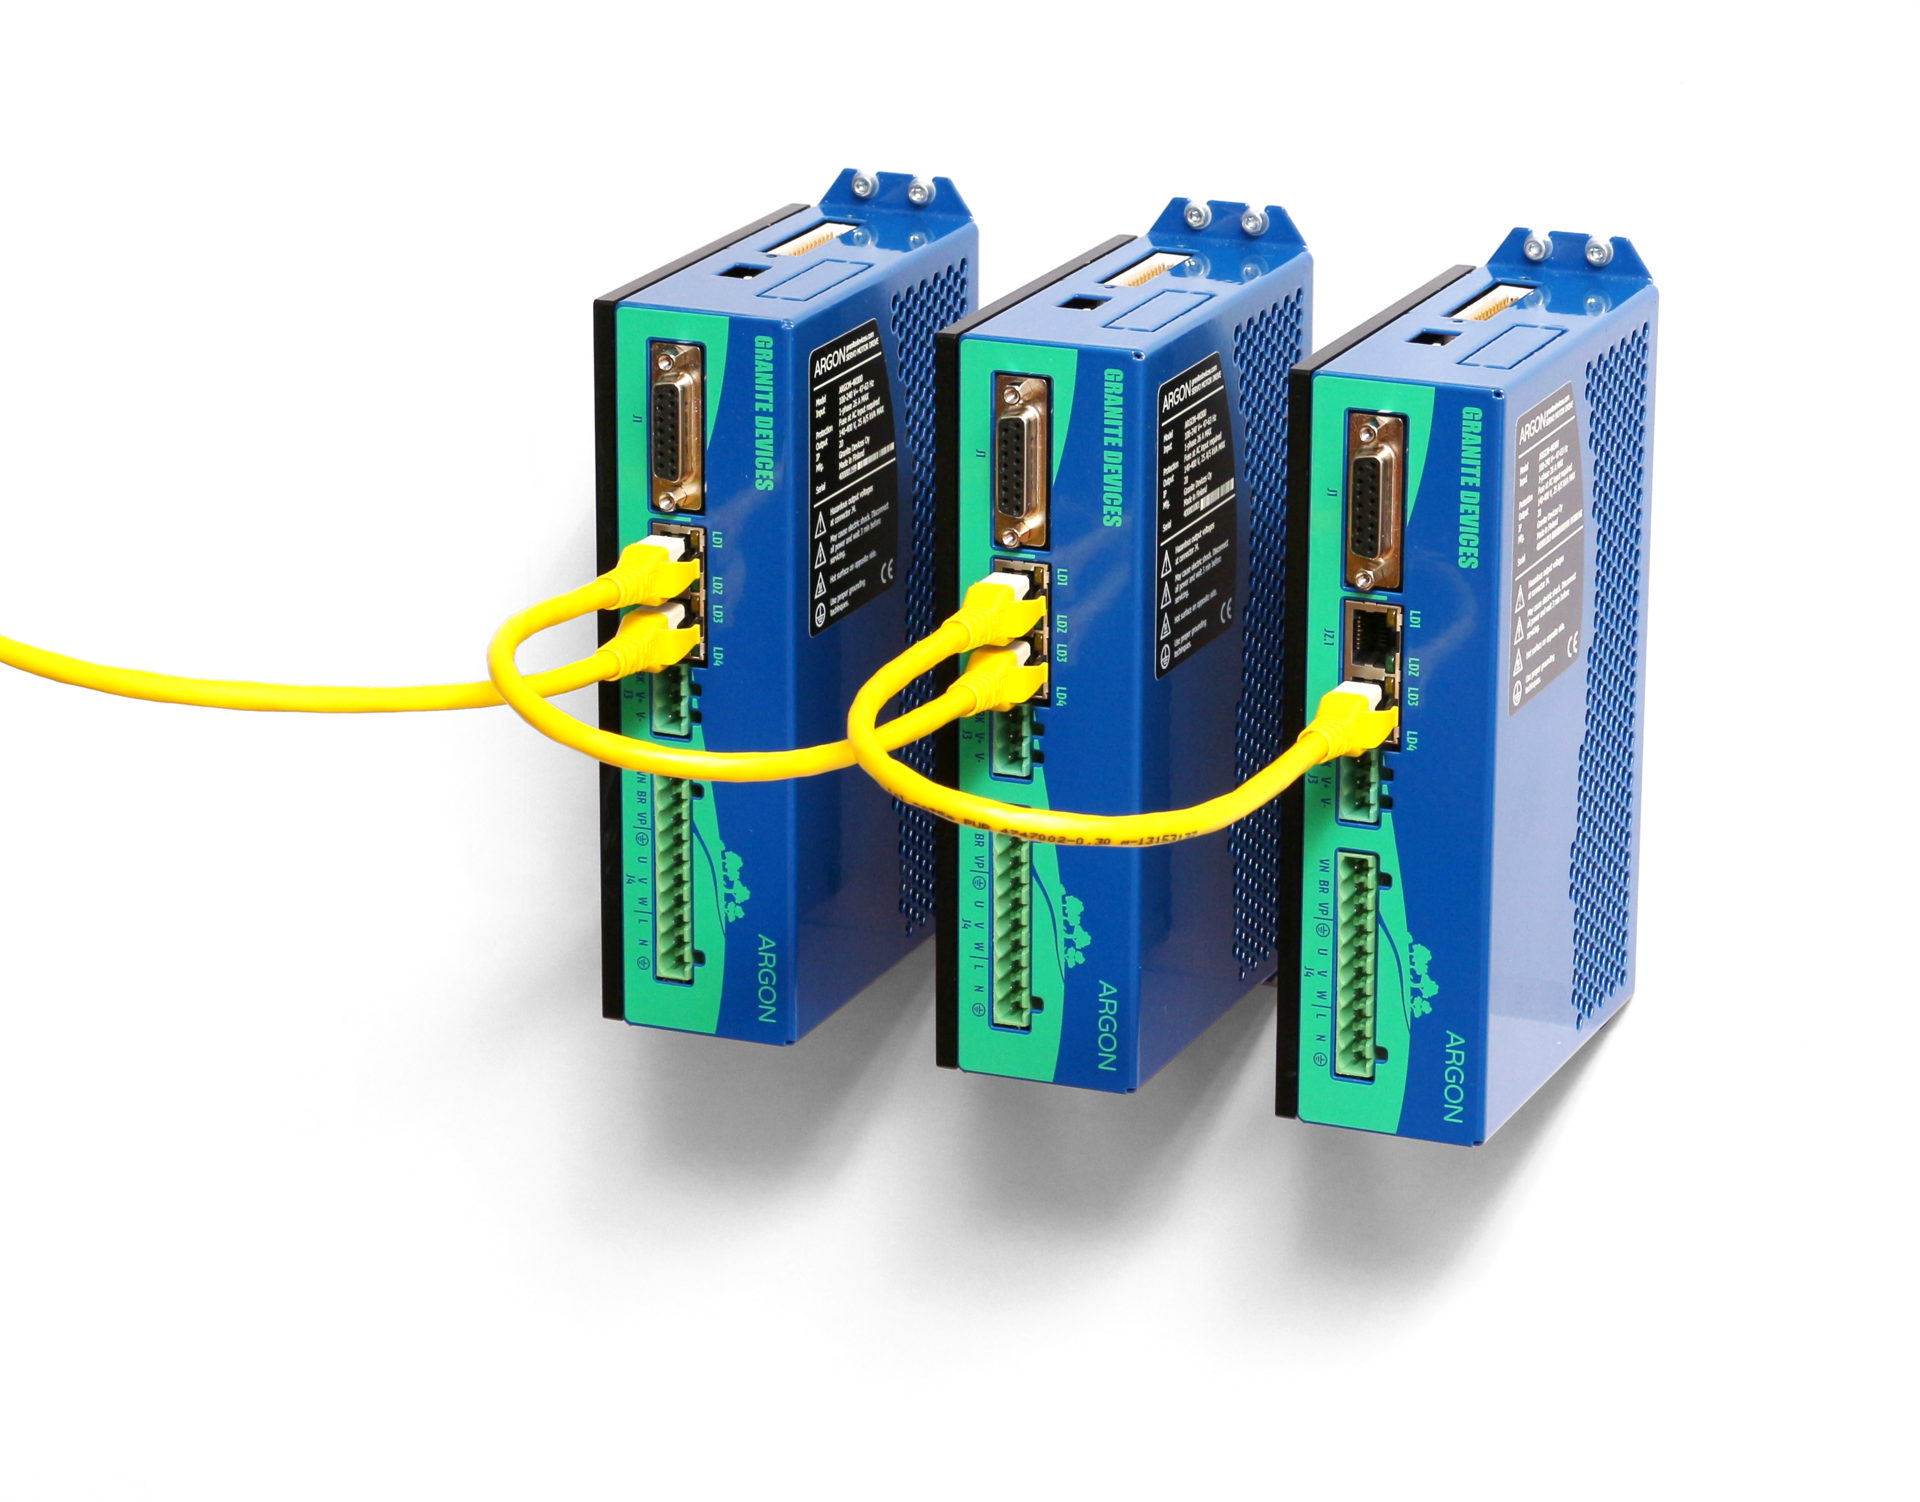
\includegraphics[height=3.6cm]{../../figures/d2_servo_drives.png}\\
\credit{Tero Kontkanen, CC BY-SA 3.0, via Wikimedia Commons}\\[1mm]
\footnotesize Servo drives: today's PID loops live inside these boxes.
\end{columns}
\end{frame}

% ---------------------------------------------------------------------
\begin{frame}{Figure credits}
\fontsize{7}{8.5}\selectfont
All other drawings and plots: own work (TikZ / circuitikz / pgfplots; numerical data in \texttt{w1d3/data/}).\\[2mm]
\begin{tabularx}{\textwidth}{@{}lXll@{}}
\toprule
File & Source (Wikimedia Commons) & Author & License\\
\midrule
d4\_kuka\_robot.jpg & File:KUKA industrial robotic arm performing ``The Beach'' by Roy Nachum - 02.jpg & Oleg Yunakov & CC BY-SA 4.0\\
d2\_governor.jpg & File:Centrifugal governor (Heat Engines, 1913).jpg & Andy Dingley (scan) & Public domain\\
d2\_bode\_portrait.png & File:Hendrik Wade Bode.png & unknown author & Public domain\\
d2\_harmonic\_drive.jpg & File:Harmonic Drive AG strain wave gear set.jpg & Pieceofmetalwork & CC BY-SA 4.0\\
d2\_pid\_controllers.jpg & File:Industrial PID controllers - front display.jpg & Bitjungle & CC BY-SA 4.0\\
d2\_servo\_drives.png & File:Servo motor drive.png & Tero Kontkanen & CC BY-SA 3.0\\
\bottomrule
\end{tabularx}
\end{frame}

% ---------------------------------------------------------------------
\begin{frame}{References}
\fontsize{7}{8.5}\selectfont
\begin{columns}[T]
\column{.5\textwidth}
\begin{itemize}
  \item K.\ Ogata, \emph{Modern Control Engineering}, 5th ed., Prentice Hall, 2010.
  \item G.\,F.\ Franklin, J.\,D.\ Powell, A.\ Emami-Naeini, \emph{Feedback Control of Dynamic Systems}, 8th ed., Pearson, 2019.
  \item K.\,J.\ \AA str\"om, R.\,M.\ Murray, \emph{Feedback Systems: An Introduction for Scientists and Engineers}, Princeton Univ.\ Press, 2008.
  \item K.\,J.\ \AA str\"om, T.\ H\"agglund, \emph{Advanced PID Control}, ISA, 2006.
  \item G.\ Ellis, \emph{Control System Design Guide}, 4th ed., Butterworth-Heinemann, 2012.
\end{itemize}
\column{.5\textwidth}
\begin{itemize}
  \item M.\,W.\ Spong, S.\ Hutchinson, M.\ Vidyasagar, \emph{Robot Modeling and Control}, 2nd ed., Wiley, 2020.
  \item J.\,J.\ Craig, \emph{Introduction to Robotics: Mechanics and Control}, 4th ed., Pearson, 2018.
  \item S.\ Skogestad, ``Simple analytic rules for model reduction and PID controller tuning,'' \emph{J.\ Process Control} 13, 291--309, 2003.
  \item J.\,G.\ Ziegler, N.\,B.\ Nichols, ``Optimum settings for automatic controllers,'' \emph{Trans.\ ASME} 64, 759--768, 1942.
  \item J.\,C.\ Maxwell, ``On governors,'' \emph{Proc.\ Royal Society of London} 16, 270--283, 1868.
\end{itemize}
\end{columns}
\end{frame}

\end{document}
